\documentclass[a4paper,11.5pt]{article}
\usepackage[textwidth=170mm, textheight=230mm, inner=20mm, top=20mm, bottom=30mm]{geometry}
\usepackage[normalem]{ulem}
\usepackage[utf8]{inputenc}
\usepackage[T1]{fontenc}
\PassOptionsToPackage{defaults=hu-min}{magyar.ldf}
\usepackage{pgfplots}
\pgfplotsset{compat=1.10}
\usepgfplotslibrary{fillbetween}
\usepackage[magyar]{babel}
\usepackage{amsmath, amsthm,amssymb,paralist,array, ellipsis, graphicx, float, bigints,tikz}
%\usepackage{marvosym}

\makeatletter
\renewcommand*{\mathellipsis}{%
	\mathinner{%
		\kern\ellipsisbeforegap%
		{\ldotp}\kern\ellipsisgap
		{\ldotp}\kern\ellipsisgap%
		{\ldotp}\kern\ellipsisaftergap%
	}%
}
\renewcommand*{\dotsb@}{%
	\mathinner{%
		\kern\ellipsisbeforegap%
		{\cdotp}\kern\ellipsisgap%
		{\cdotp}\kern\ellipsisgap%
		{\cdotp}\kern\ellipsisaftergap%
	}%
}
\renewcommand*{\@cdots}{%
	\mathinner{%
		\kern\ellipsisbeforegap%
		{\cdotp}\kern\ellipsisgap%
		{\cdotp}\kern\ellipsisgap%
		{\cdotp}\kern\ellipsisaftergap%
	}%
}
\renewcommand*{\ellipsis@default}{%
	\ellipsis@before
	\kern\ellipsisbeforegap
	.\kern\ellipsisgap
	.\kern\ellipsisgap
	.\kern\ellipsisgap
	\ellipsis@after\relax}
\renewcommand*{\ellipsis@centered}{%
	\ellipsis@before
	\kern\ellipsisbeforegap
	.\kern\ellipsisgap
	.\kern\ellipsisgap
	.\kern\ellipsisaftergap
	\ellipsis@after\relax}
\AtBeginDocument{%
	\DeclareRobustCommand*{\dots}{%
		\ifmmode\@xp\mdots@\else\@xp\textellipsis\fi}}
\def\ellipsisgap{.1em}
\def\ellipsisbeforegap{.05em}
\def\ellipsisaftergap{.05em}
\makeatother

\usepackage{hyperref}
\hypersetup{
	colorlinks = true	
}

\DeclareMathOperator{\Int}{int}
\DeclareMathOperator{\tg}{tg}
\DeclareMathOperator{\ctg}{ctg}
\DeclareMathOperator{\Th}{th}
\DeclareMathOperator{\sh}{sh}
\DeclareMathOperator{\ch}{ch}
\DeclareMathOperator{\arsh}{arsh}
\DeclareMathOperator{\arch}{arch}
\DeclareMathOperator{\arth}{arth}
\DeclareMathOperator{\arcth}{arcth}
\DeclareMathOperator{\grad}{grad}
\DeclareMathOperator{\arc}{arc}
\DeclareMathOperator{\arctg}{arc tg}
\DeclareMathOperator{\arcctg}{arc ctg}
\newcommand{\norm}[1]{\left\lVert#1\right\rVert}

\begin{document}
	%%%%%%%%%%%RÖVIDÍTÉSEK%%%%%%%%%%
	\setlength\parindent{0pt}
	\def\a{\textbf{a}}
	\def\b{\textbf{b}}
	\def\N{\hskip 10 true mm}
	\def\a{\textbf{a}}
	\def\b{\textbf{b}}
	\def\c{\textbf{c}}
	\def\d{\textbf{d}}
	\def\e{\textbf{e}}
	\def\gg{$\gamma$}
	\def\vi{\textbf{i}}
	\def\jj{\textbf{j}}
	\def\kk{\textbf{k}}
	\def\fh{\overrightarrow}
	\def\l{\lambda}
	\def\m{\mu}
	\def\v{\textbf{v}}
	\def\0{\textbf{0}}
	\def\s{\hspace{0.2mm}\vphantom{\beta}}
	\def\Z{\mathbb{Z}}
	\def\Q{\mathbb{Q}}
	\def\R{\mathbb{R}}
	\def\C{\mathbb{C}}
	\def\N{\mathbb{N}}
	\def\Rn{\mathbb{R}^{n}}
	\def\Ra{\overline{\mathbb{R}}}
	\def\sume{\displaystyle\sum_{n=1}^{+\infty}}
	\def\sumn{\displaystyle\sum_{n=0}^{+\infty}}
	\def\biz{\emph{Bizonyítás:\ }}
	\def\narrow{\underset{n\rightarrow+\infty}{\longrightarrow}}
	\def\limn{\displaystyle\lim_{n\to +\infty}}
	%	\def\definition{\textbf{Definíció:\ }}
	%	\def\theorem{\textbf{Tétel:\ }}
	%\def\note{\emph{Megjegyzés:\ }}
	%\def\example{\textbf{Példa:\ }} 
	
	\theoremstyle{definition}
	\newtheorem{theorem}{Tétel}[subsubsection] % reset theorem numbering for each chapter
	
	\theoremstyle{definition}
	\newtheorem{definition}[theorem]{Definíció} % definition numbers are dependent on theorem numbers
	\newtheorem{example}[theorem]{Példa} % same for example numbers
	\newtheorem{exercise}[theorem]{Házi feladat} % same for example numbers
	\newtheorem{note}[theorem]{Megjegyzés} % same for example numbers
	\newtheorem{task}[theorem]{Feladat} % same for example numbers
	\newtheorem{revision}[theorem]{Emlékeztető} % same for example numbers
	%%%%%%%%%%%%%%%%%%%%%%%%%%%%%%%%%
	\begin{center}
		{\LARGE\textbf{Analízis 3. A szakirány}}
		\smallskip
		
		{\Large Gyakorlati jegyzet}
		
		\smallskip
		12. óra.
	\end{center}
	A jegyzetet \textsc{Umann} Kristóf készítette \textsc{Filipp} Zoltán István gyakorlatán. (\today)
	%\subsection{Folytatás}
	\begin{task}
		%TODO feladatfolytatás
		\[ f(x,y)=x^4+y^4-x^2-2xy-y^2 \]
		Megállapítottuk korábban, hogy a $(0,0)$ ponthoz kellett külön vizsgálat, lévén az általunk kapott mátrix negatív szemidefinit volt.
		\[ f(0,0)=0 \]
		
		\begin{figure}[H]
			\centering
			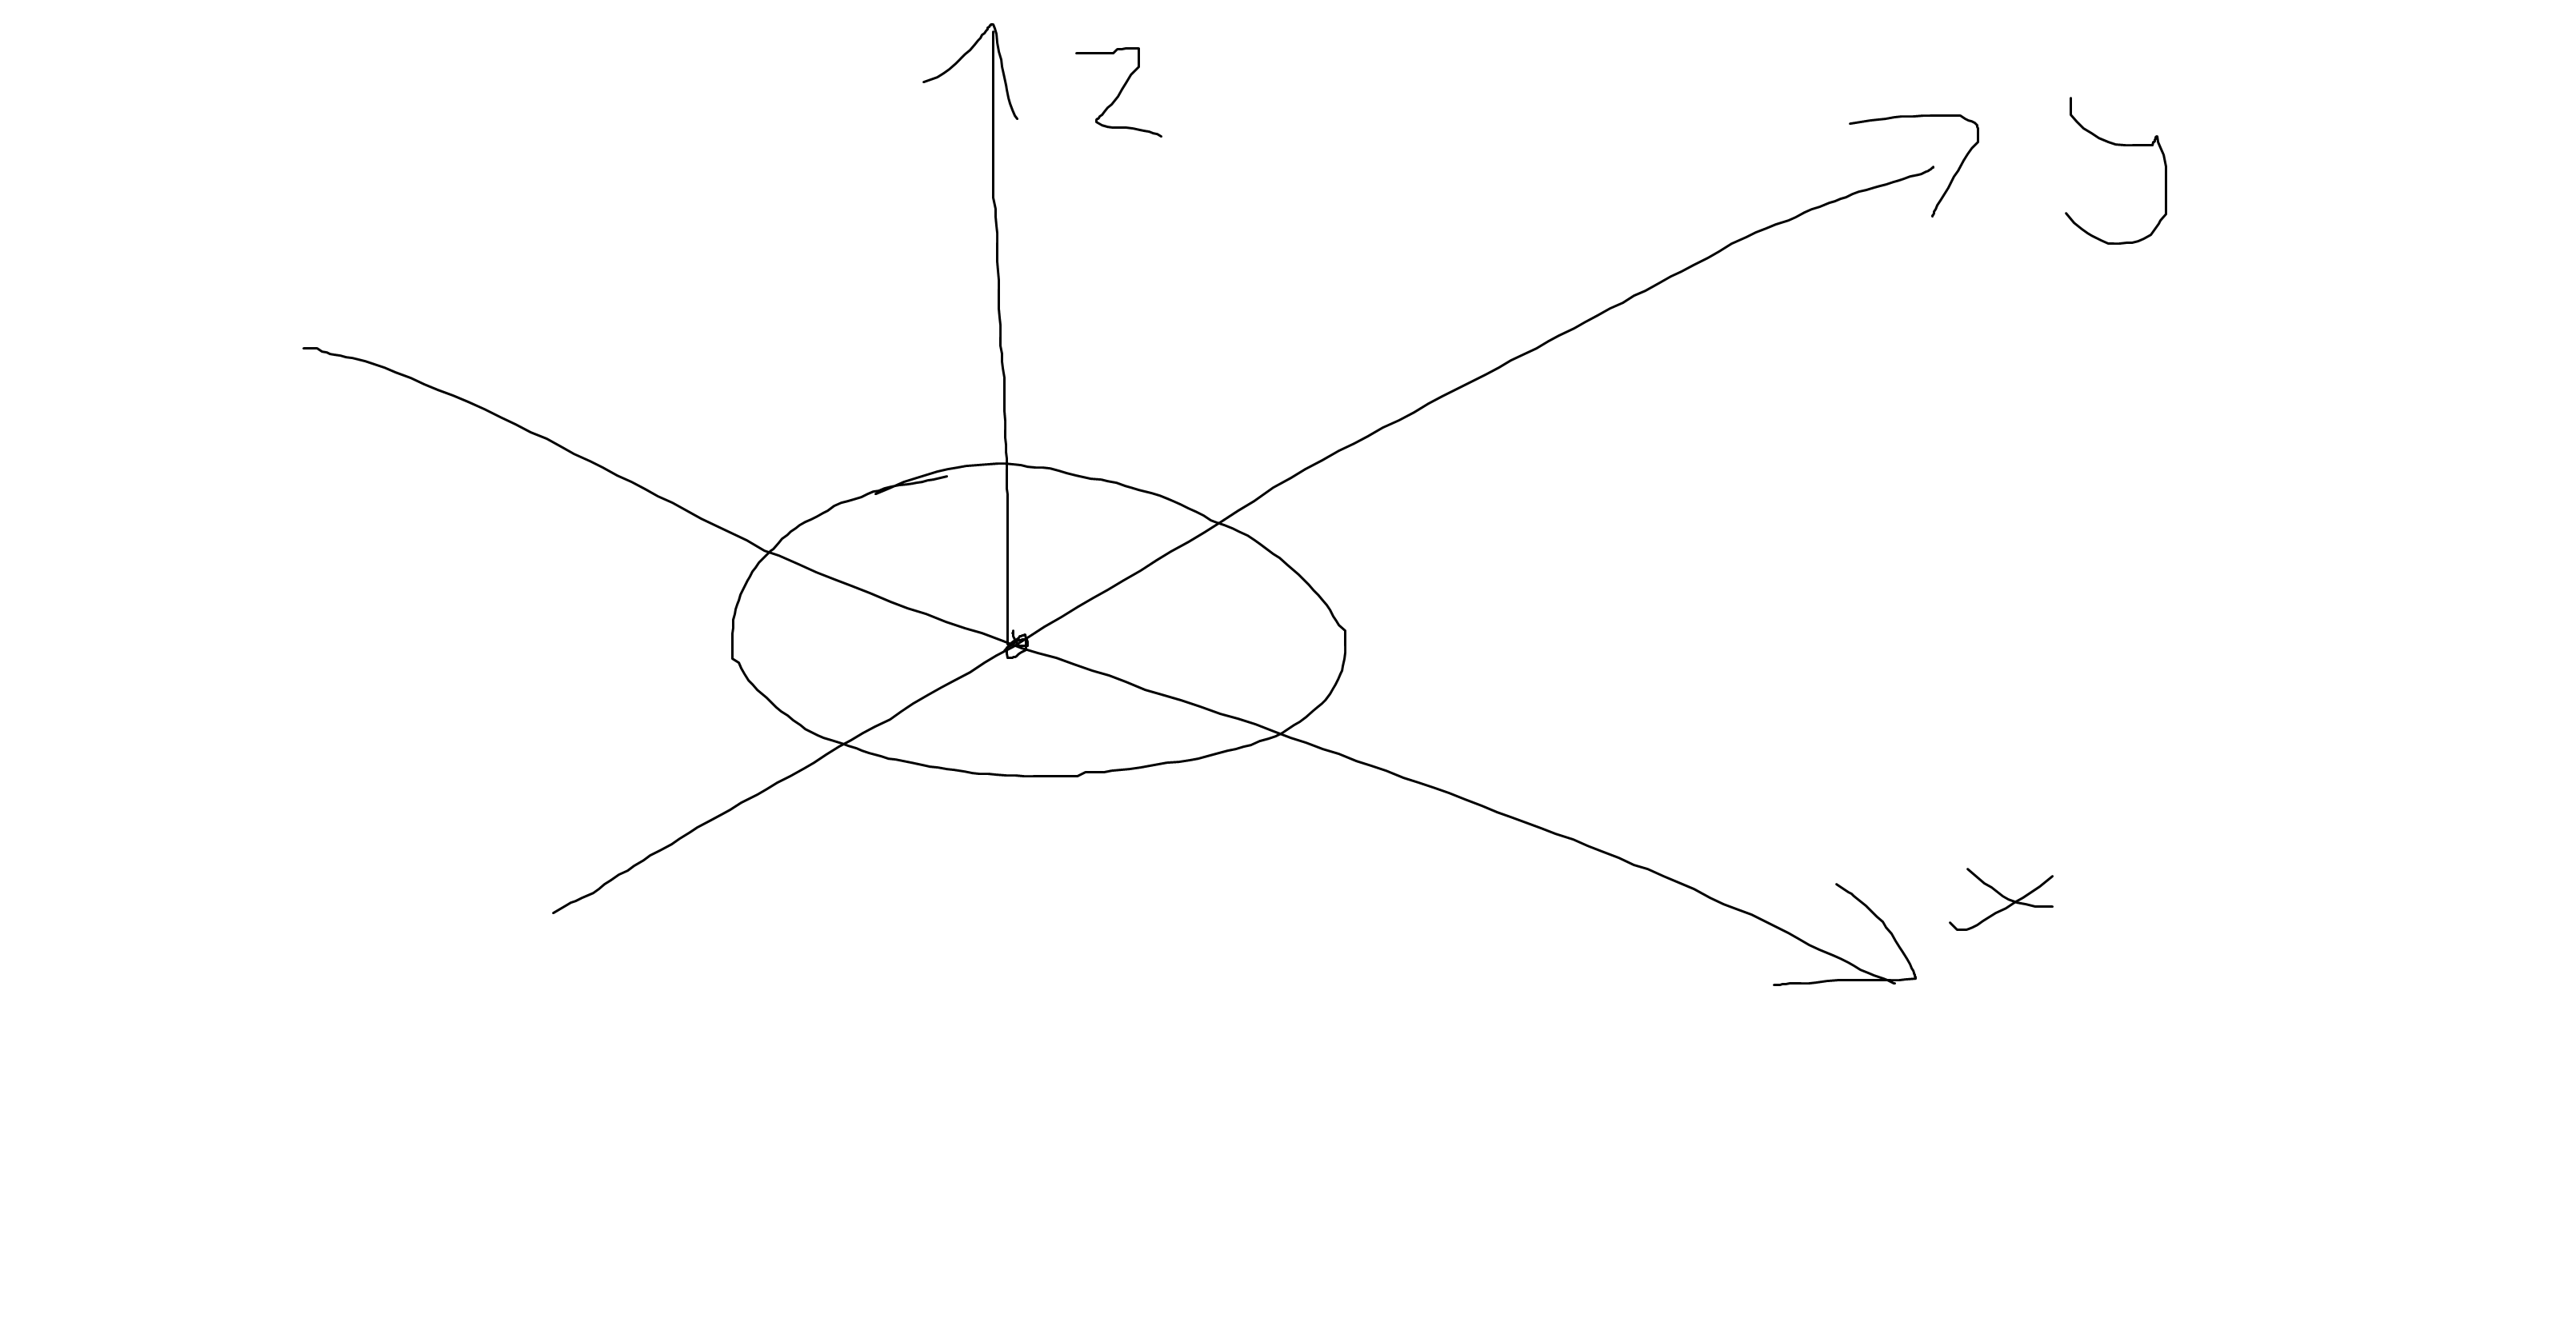
\includegraphics[height=4cm]{kepek/41.png}
			\caption{Ha (0,0) lokális minimum, akkor be kéne látunk, hogy a (0,0) körüli környezetben, melyben minden érték pozitív. Ha maximum, a környezetben negatívnak kell lennie. Ha egyik sem, akkor kell negatív és pozitív érték is.}
		\end{figure}
		\[  y=0\quad \text{mentén}\quad f(x,0)=x^4-x^2=x^2(x^2-1) \]
		\begin{figure}[H]
			\centering
			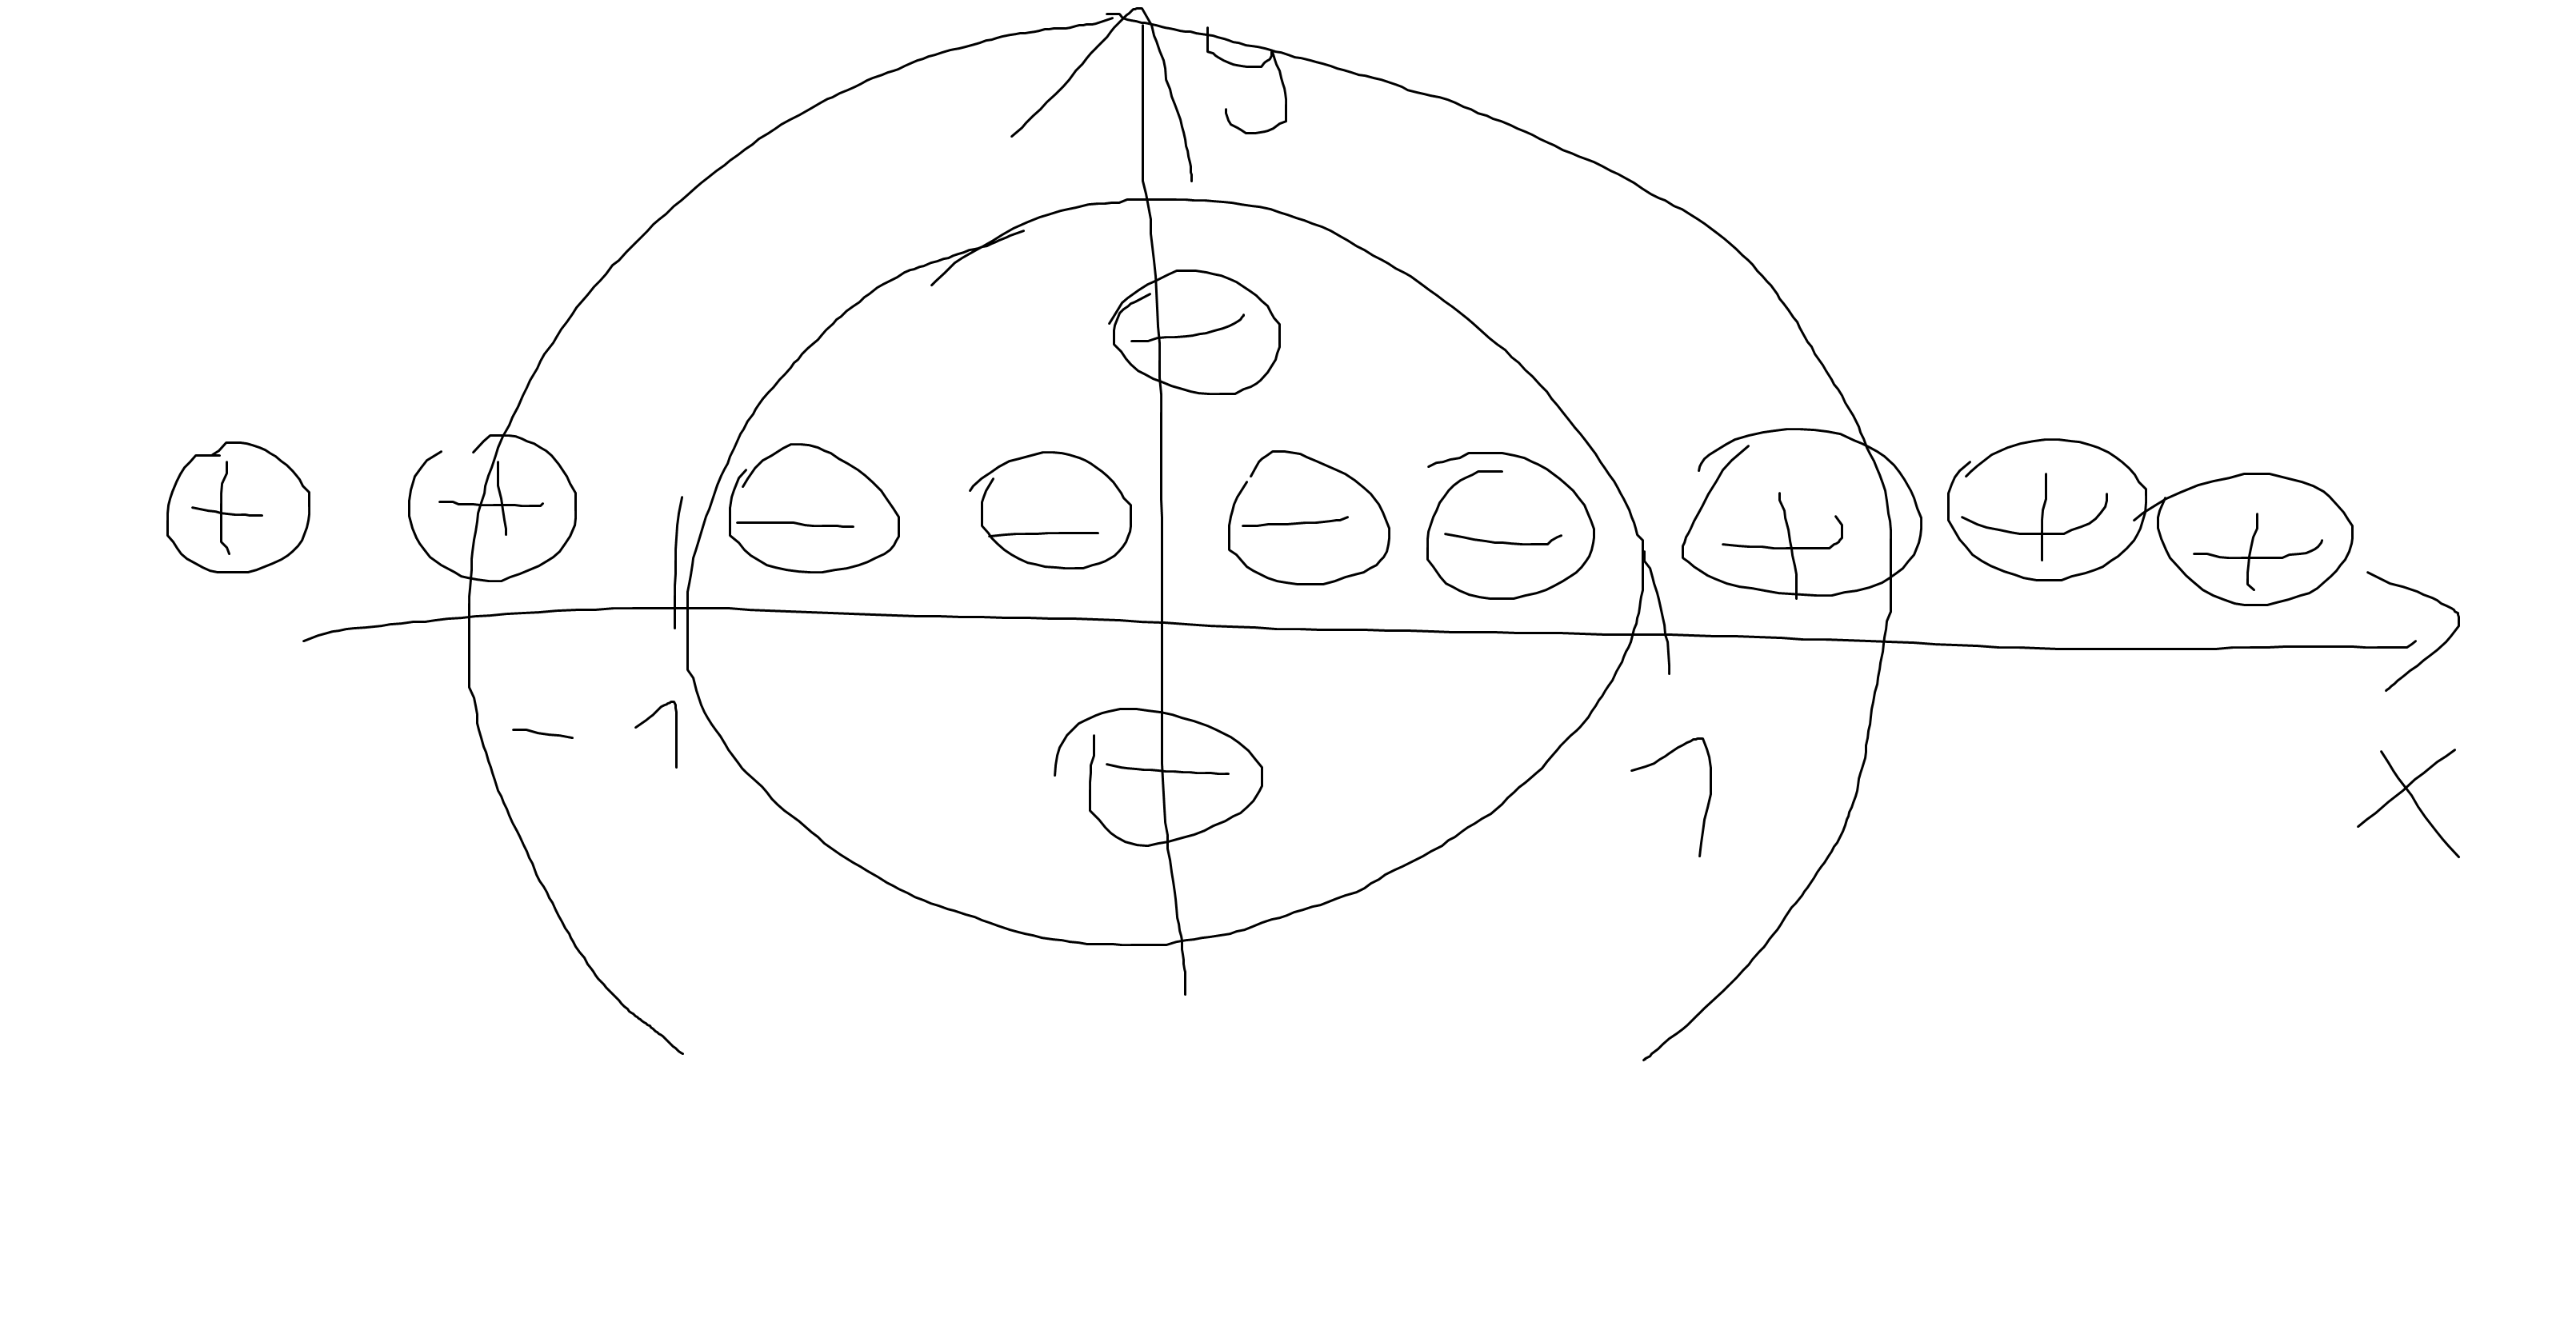
\includegraphics[height=4cm]{kepek/42.png}
			\caption{Ez alapján látszik, hogy a 0 körüli környezetnek mindig lesz olyan része, mely negatív értékeket vesz fel.}
		\end{figure}
		Próbáljunk keresni egy olyan részt ebben az 1 sugarú körben, melyben pozitív értékeket is felvesz a függvény.
		\[ f(x,y)=x^4+y^4-(x+y)^2 \]
		Ezt elérhetjük úgy, hogy a fenti képletből lenullázzuk a a $(x+y)^2$ tagot.
		\[ y=-x\quad \text{mentén}\quad f(x,-x)=2x^4>0\quad \forall x\in\R\setminus\{0\} \]
		\begin{figure}[H]
			\centering
			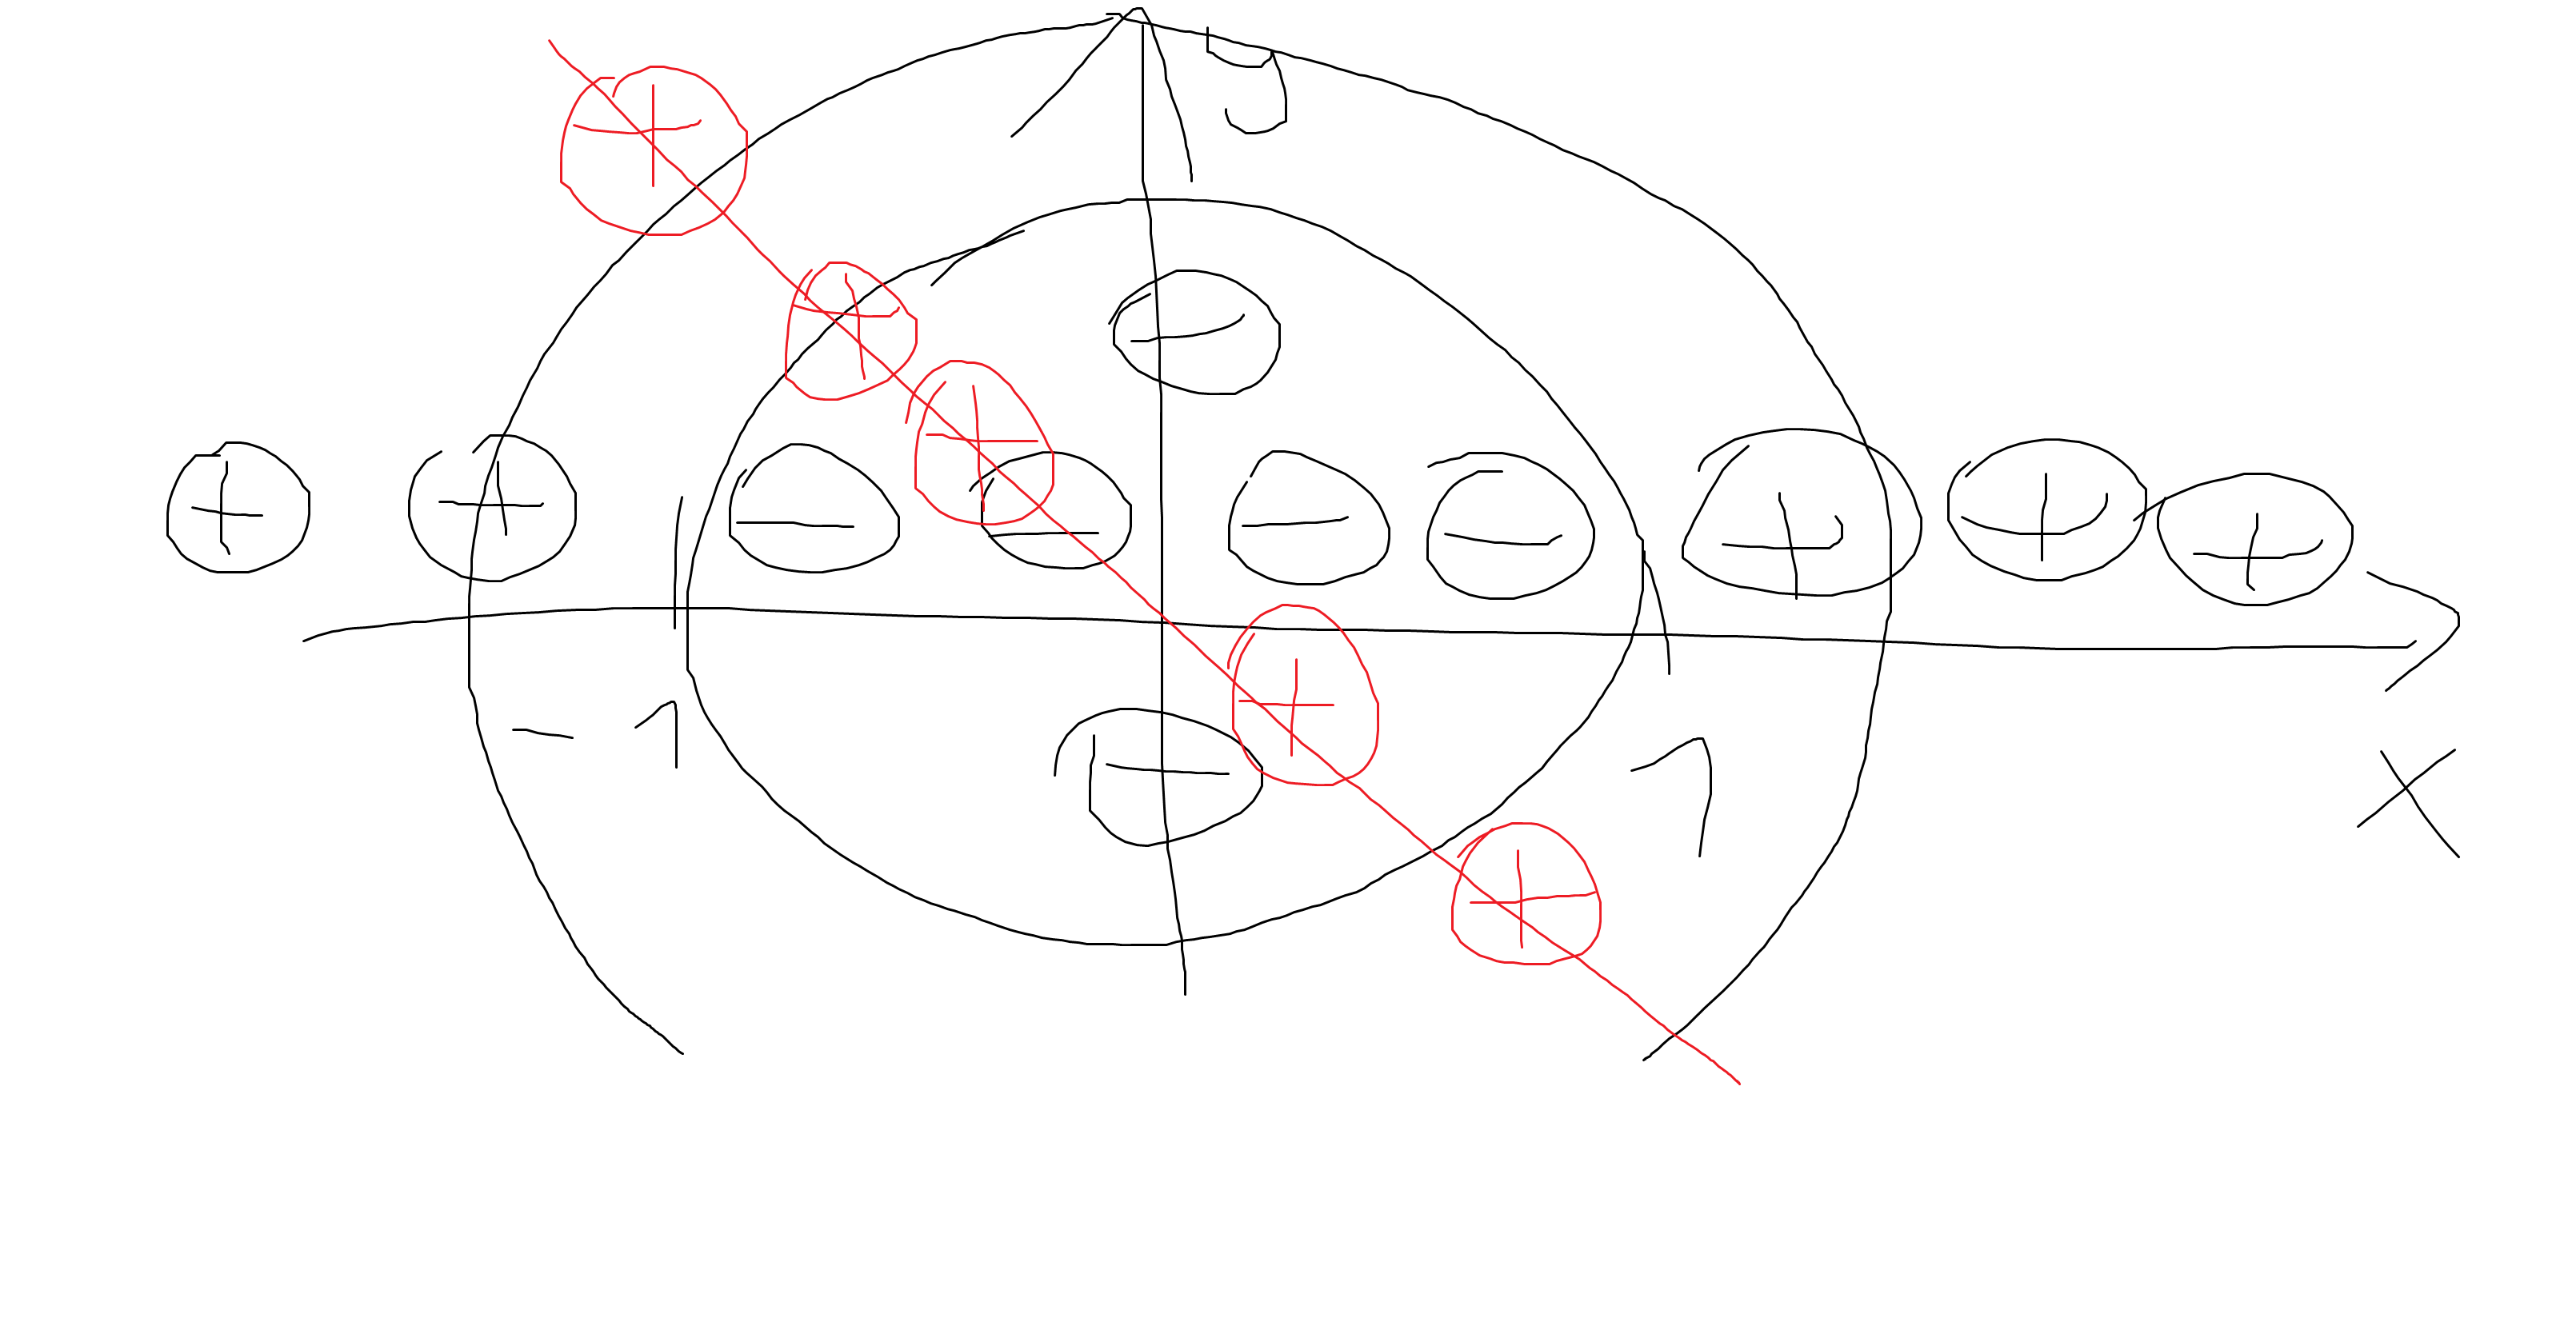
\includegraphics[height=4cm]{kepek/43.png}
			\caption{}
		\end{figure}
		Ezzel beláttuk, hogy a (0,0) pont minden környezetében találhatunk negatív és pozitív értékeket is, azaz
		
		Legyen $x_\delta:=\frac{\min\{1,\delta\}}{2}$
		\[ \forall\delta>0\quad \text{és}\quad k_\delta(0,0):\quad \overbrace{f(x_\delta,0)}^{>0}<f(0,0)=0<f\left(\frac{\delta}{2},-\frac{\delta}{2}\right)=2\cdot\frac{\delta^4}{16}=\frac{\delta^4}{8} \]
		\begin{figure}[H]
			\centering
			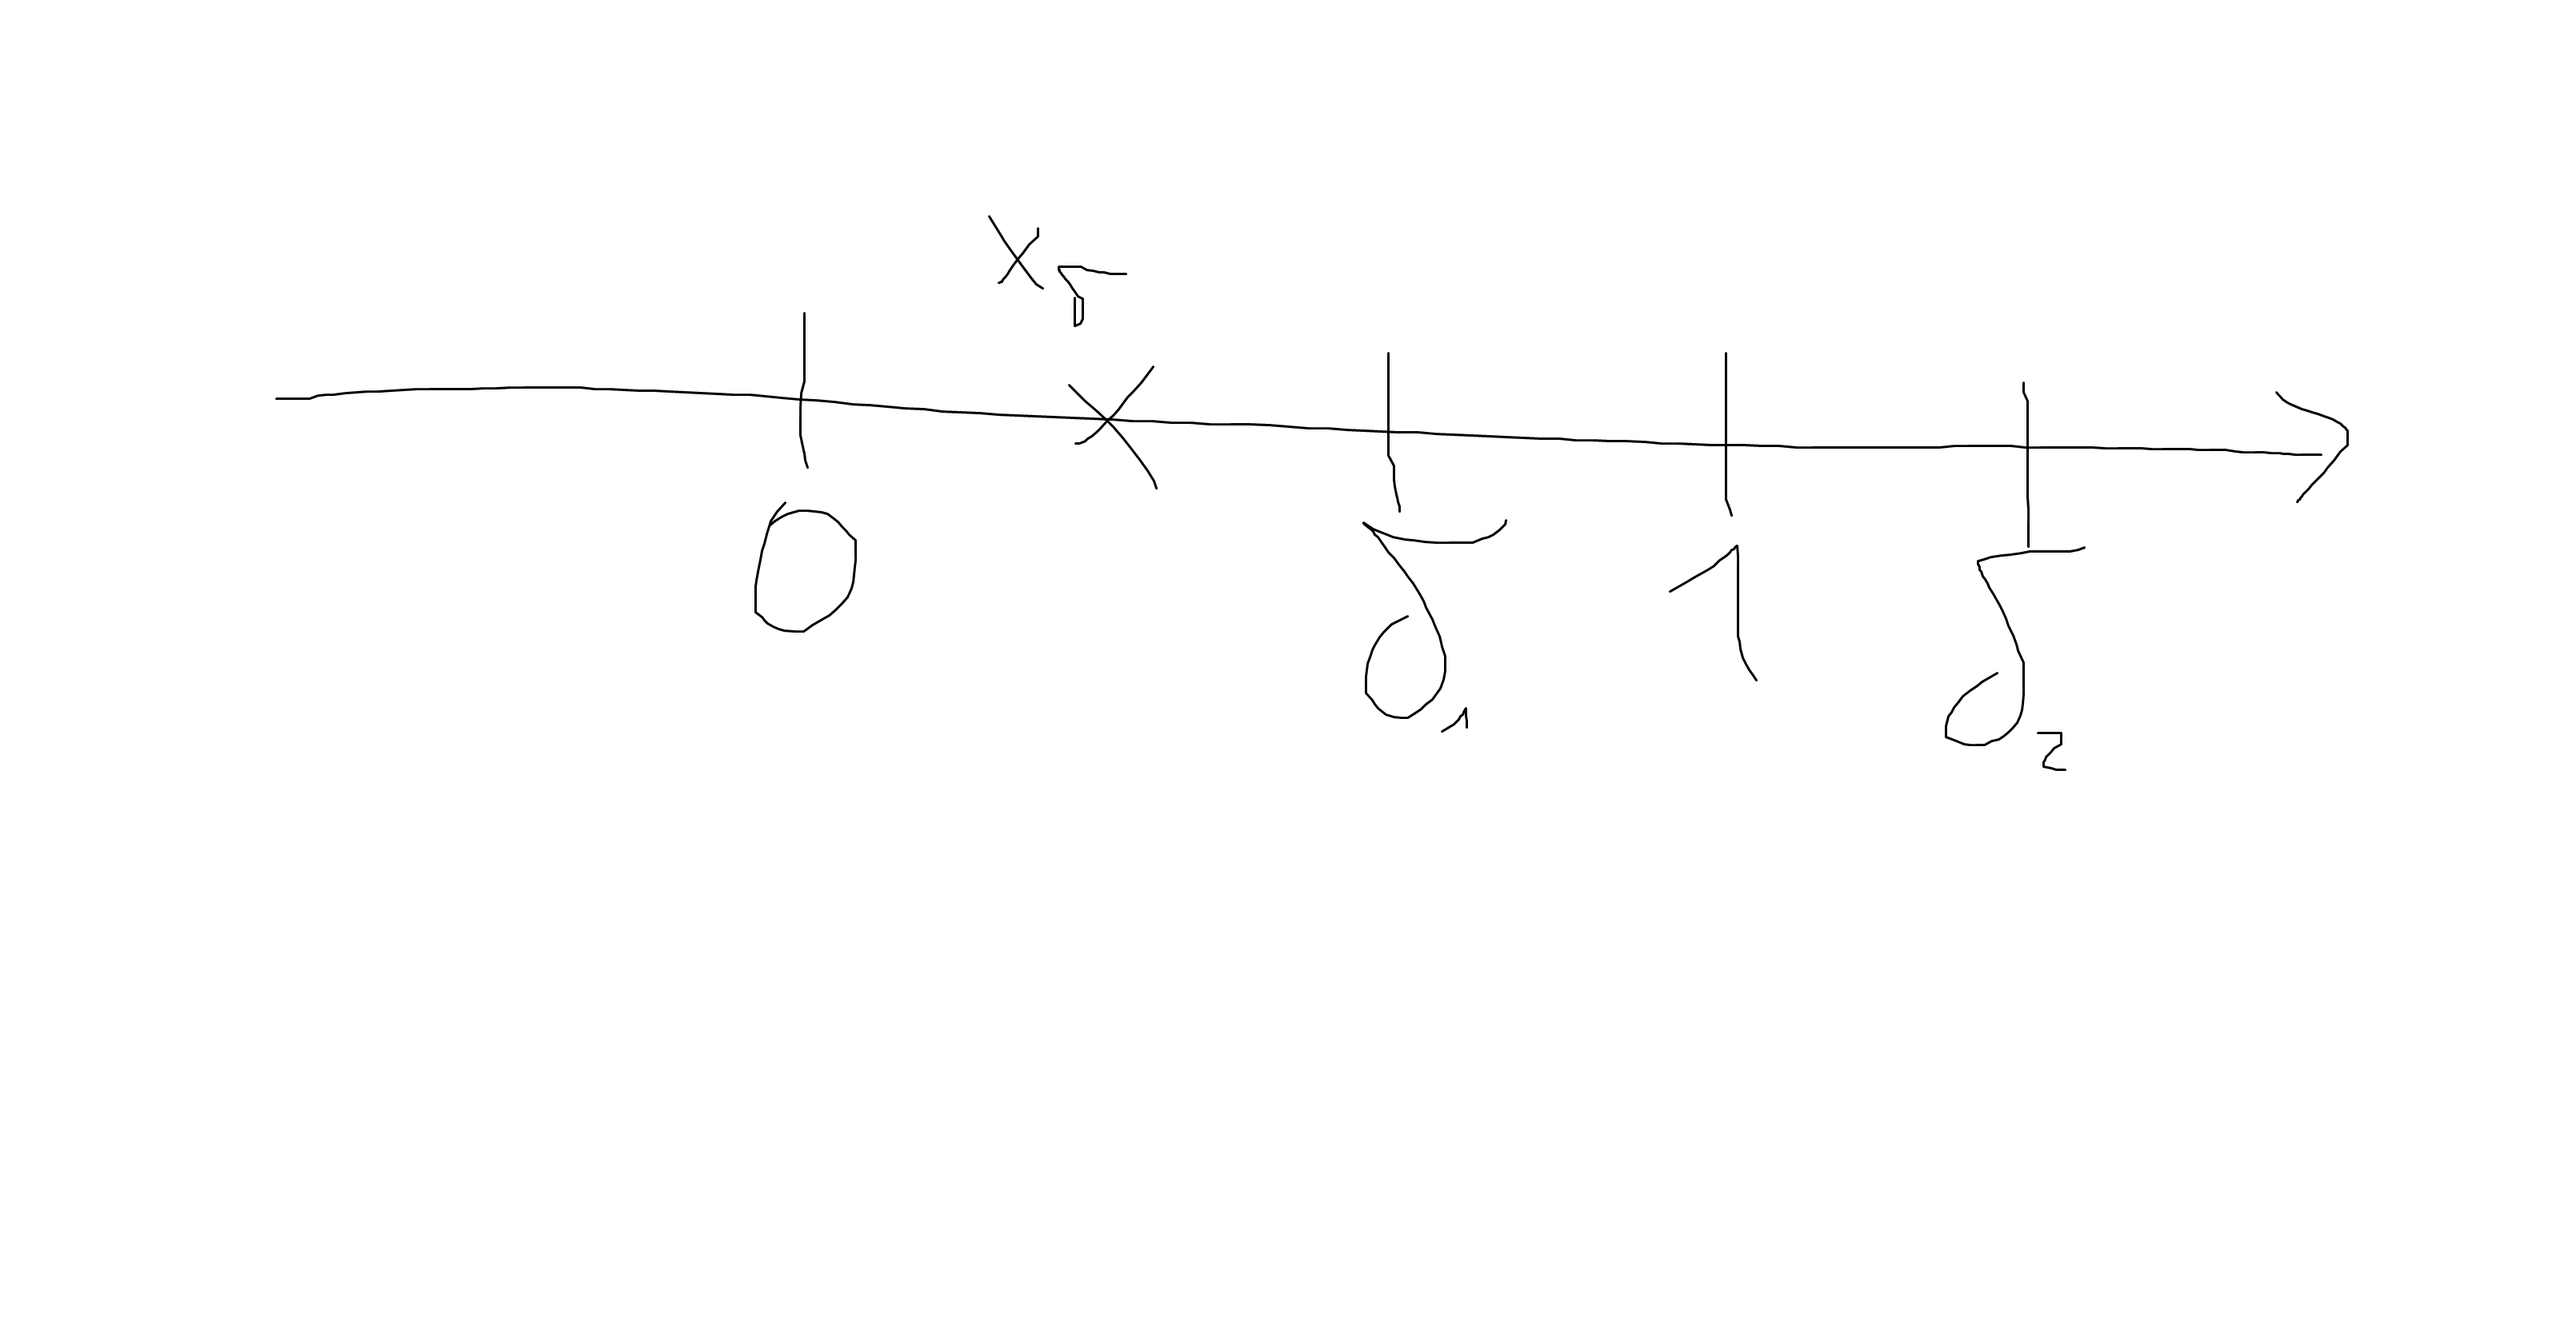
\includegraphics[height=4cm]{kepek/44.png}
			\caption{}
		\end{figure}
		$\Rightarrow \quad (0,0)$ nem lokális szélső érték hely.
	\end{task}
	\begin{task}
		\[ f(x,y):=x^4+y^2\quad ((x,y)\in\R^2) \]
		Lokális szélső értéket keresünk.
		
		\textit{Megoldás:} Első lépésben:
		\begin{align*}
			\partial_1f(x,y)=4x^3=0\\
			\partial_2f(x,y)=2y=0
		\end{align*}
		Ebből követekzik hogy $(x,y)=(0,0)$.
		
		Második lépésben?
		\[ f''(x,y)=\begin{bmatrix}
			12y^2&0\\
			0&2
		\end{bmatrix}\quad ((x,y)\in\R^2)\quad \Rightarrow\quad f''(0,0)=\begin{bmatrix}
		0&0\\
		0&2
		\end{bmatrix},\quad \varDelta_1=0,\quad \varDelta_2=0 \]
		Ismét nem működnek a tételek, további vizsgálatra van szükség.
		\[ f(0,0)=0\leq x^4+y^2=f(x,y)\quad (\forall(x,y)\in\R^2)\quad \Rightarrow\quad \text{abszolút minimum hely.} \]
	\end{task}
	\begin{task}
		\[ f(x,y)=x^3+y^2\quad ((x,y)\in\R^2) \]
		\textit{Megoldás:} Első lépésben
		\begin{align*}
			\partial_1f(x,y)=3x^2=0\\
			\partial_2f(x,y)=2y=0
		\end{align*}
		Azaz $(x,y)=(0,0)$.
		
		Második lépésben:
		\[ f''(x,y)=\begin{bmatrix}
			6x&0\\
			0&2
		\end{bmatrix}\quad \Rightarrow\quad f''(0,0)=\begin{bmatrix}
			0&0\\
			0&2
		\end{bmatrix} \]
		Tételek ismét nem máködnek, tovább kell vizsgálni (0,0)-t. Kínálja magát az $y=0$ irány:
		\[ f(x,y)=x^3\quad \Rightarrow\quad f(x,0)=x^3=\begin{cases}
			>0\quad x>0\\
			<0\quad x<0
		\end{cases} \]
		$\Rightarrow\quad \forall\delta>0$ és $k_\delta(0,0)$ környezetben:
		\[ f\left(-\frac{\delta}{2},0\right)<f(0,0)=0<f\left(\frac{\delta}{2},0\right)\quad \Rightarrow\quad \text{(0,0) nem lokális szélső érték hely.} \]
		\begin{figure}[H]
			\centering
			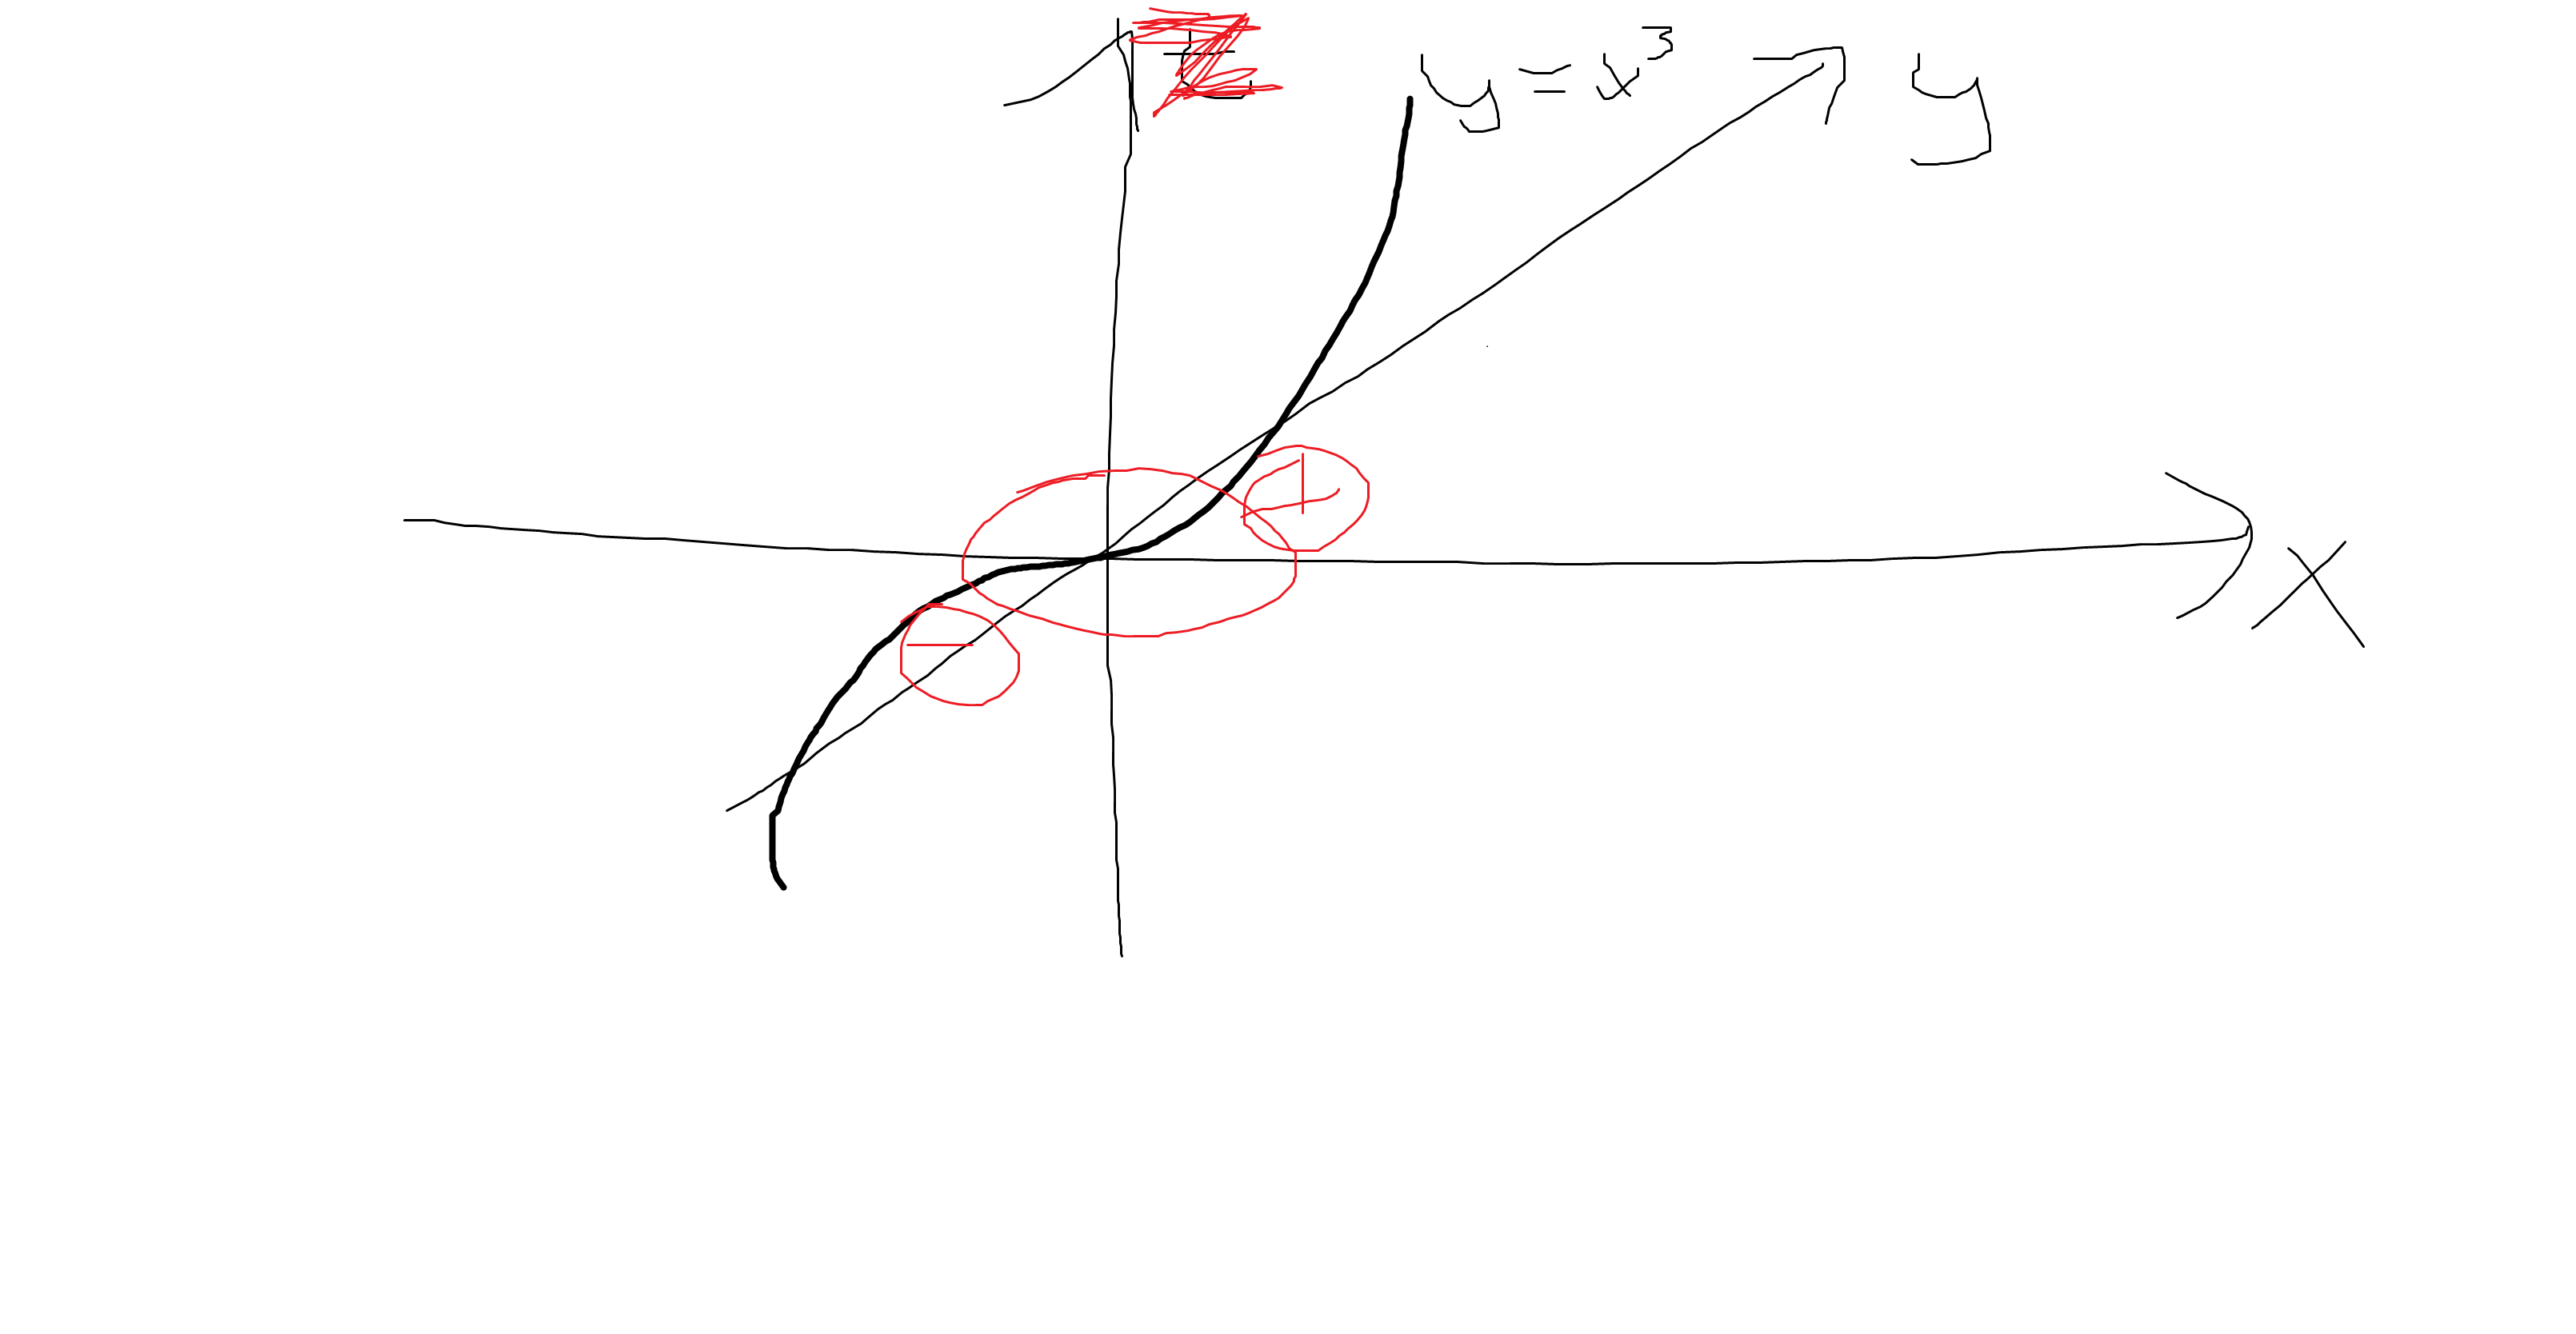
\includegraphics[height=4cm]{kepek/45.png}
			\caption{}
		\end{figure}
	\end{task}
	\subsection{Abszolút szélső érték keresés}
	\begin{task}
		\[ f(x,y):=y(2x-3)\quad ((x,y)\in A) \]
		$A$: Az $>=x^2;\quad y=0;$ és $x=2$ egyenletű götbék által határolt korlátos és zárt. Keressünk abszolút szélső értéket $A$-n.
		\begin{figure}[H]
			\centering
			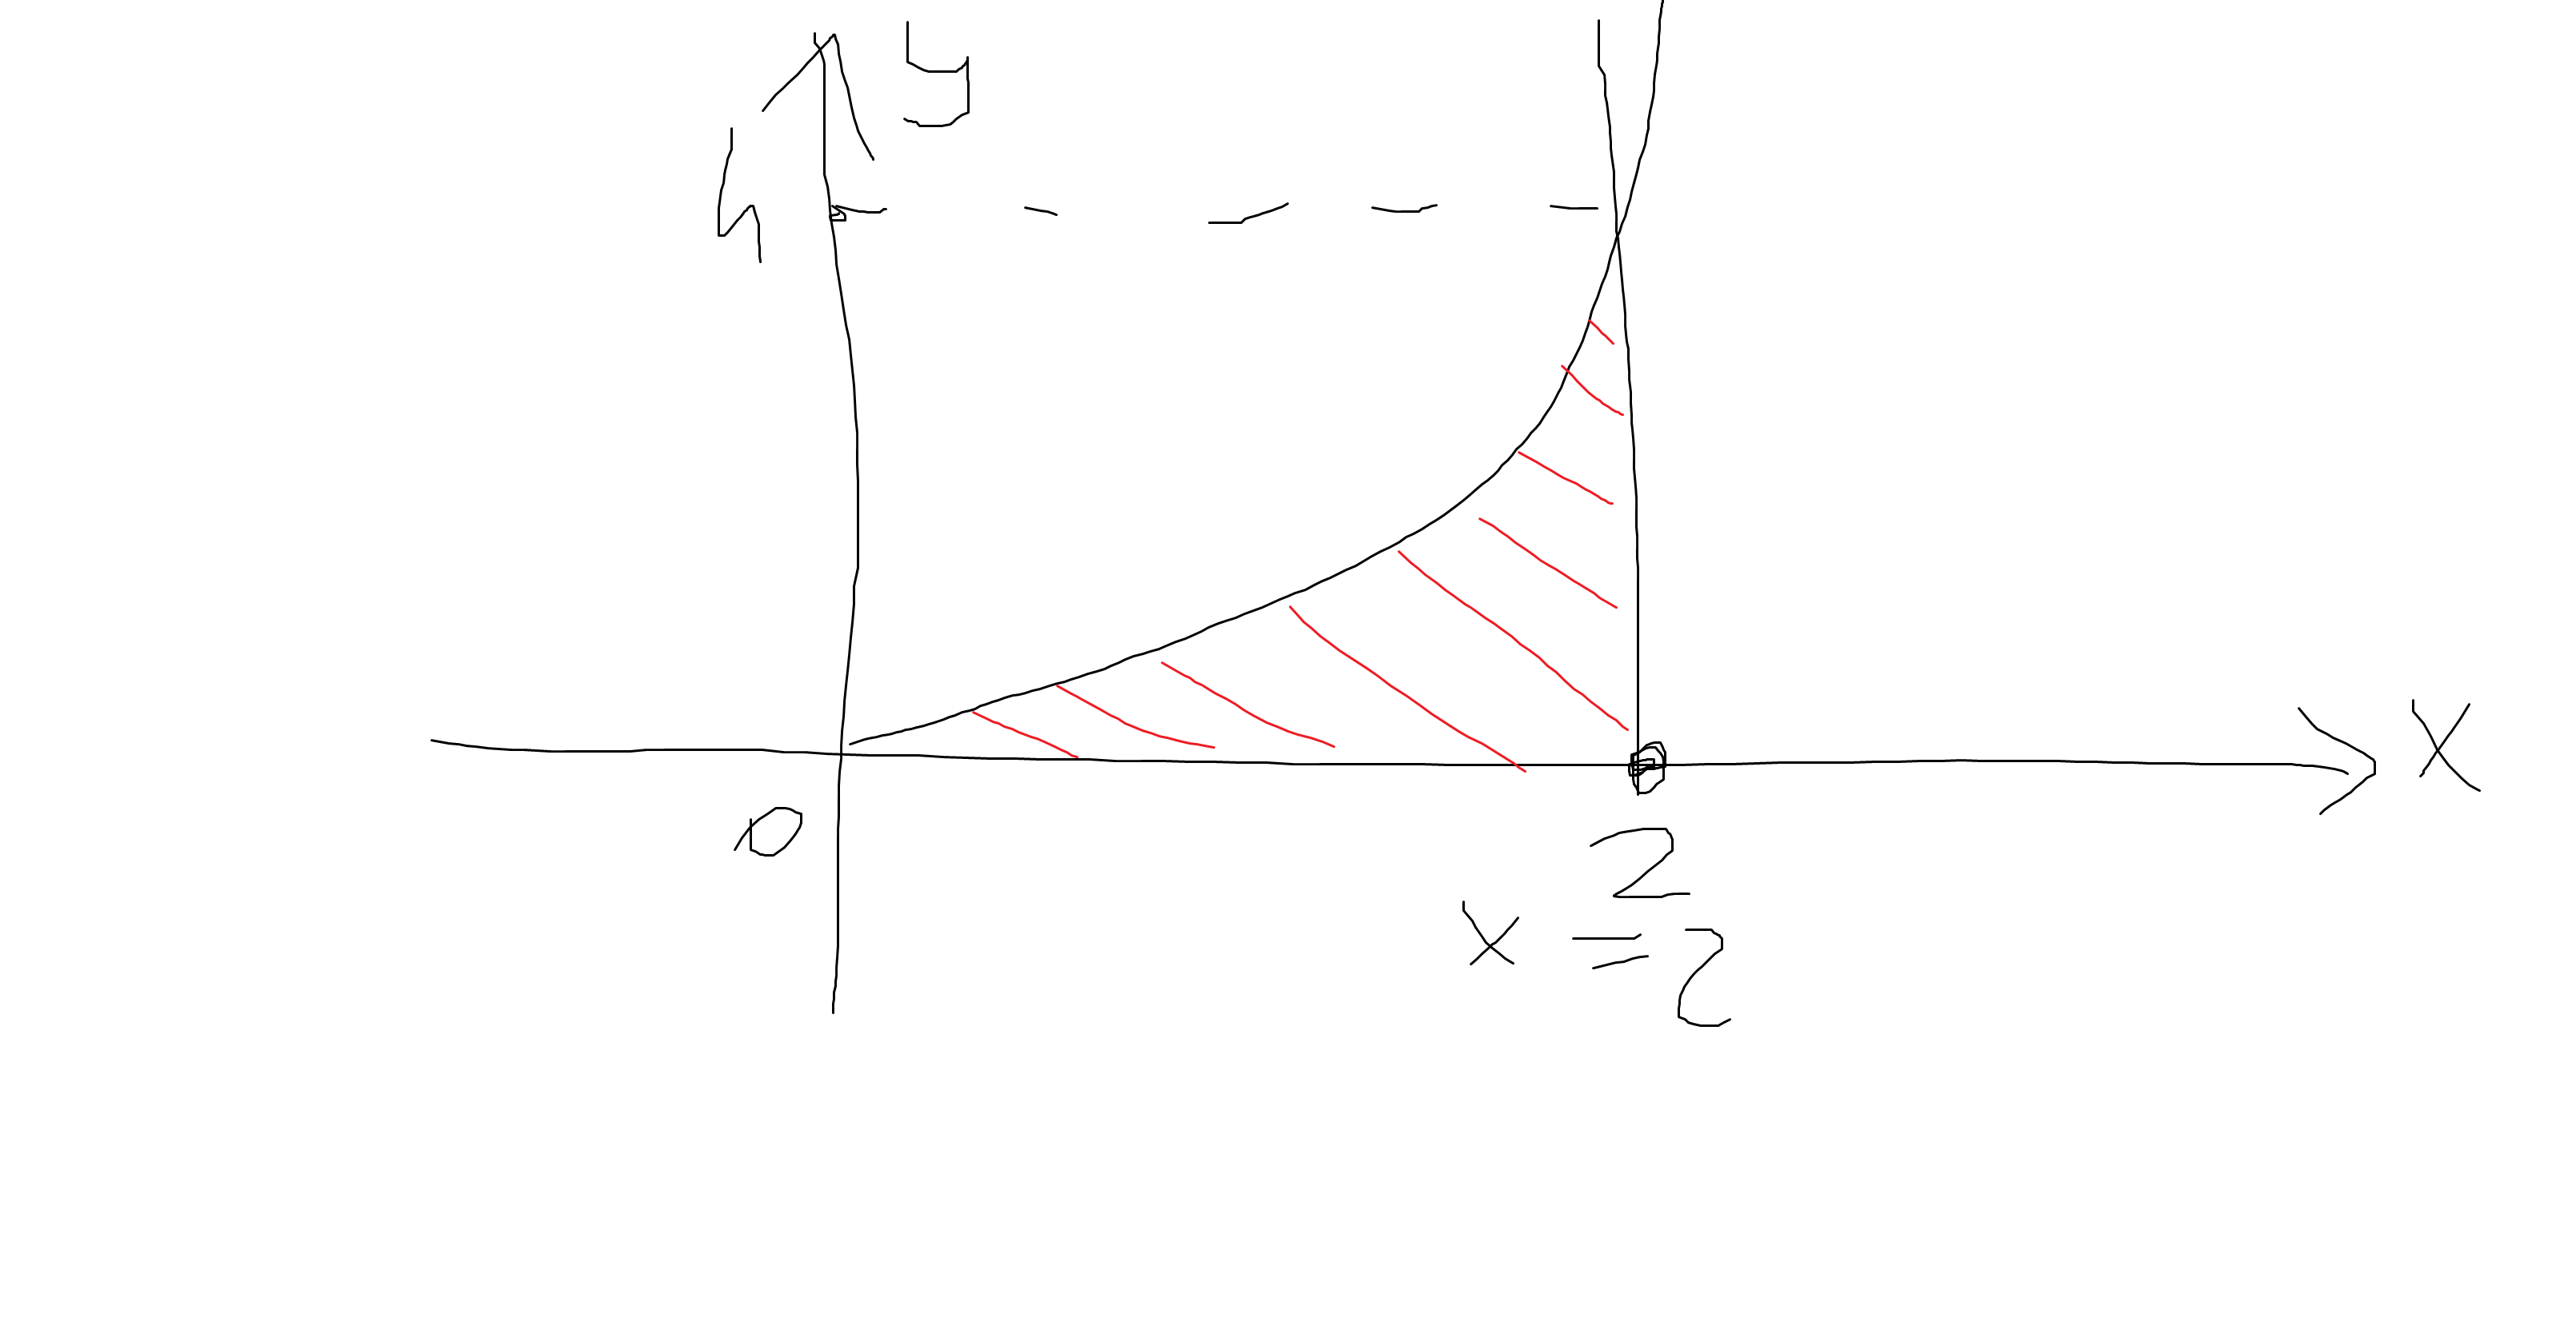
\includegraphics[height=4cm]{kepek/46.png}\quad \quad \quad 
			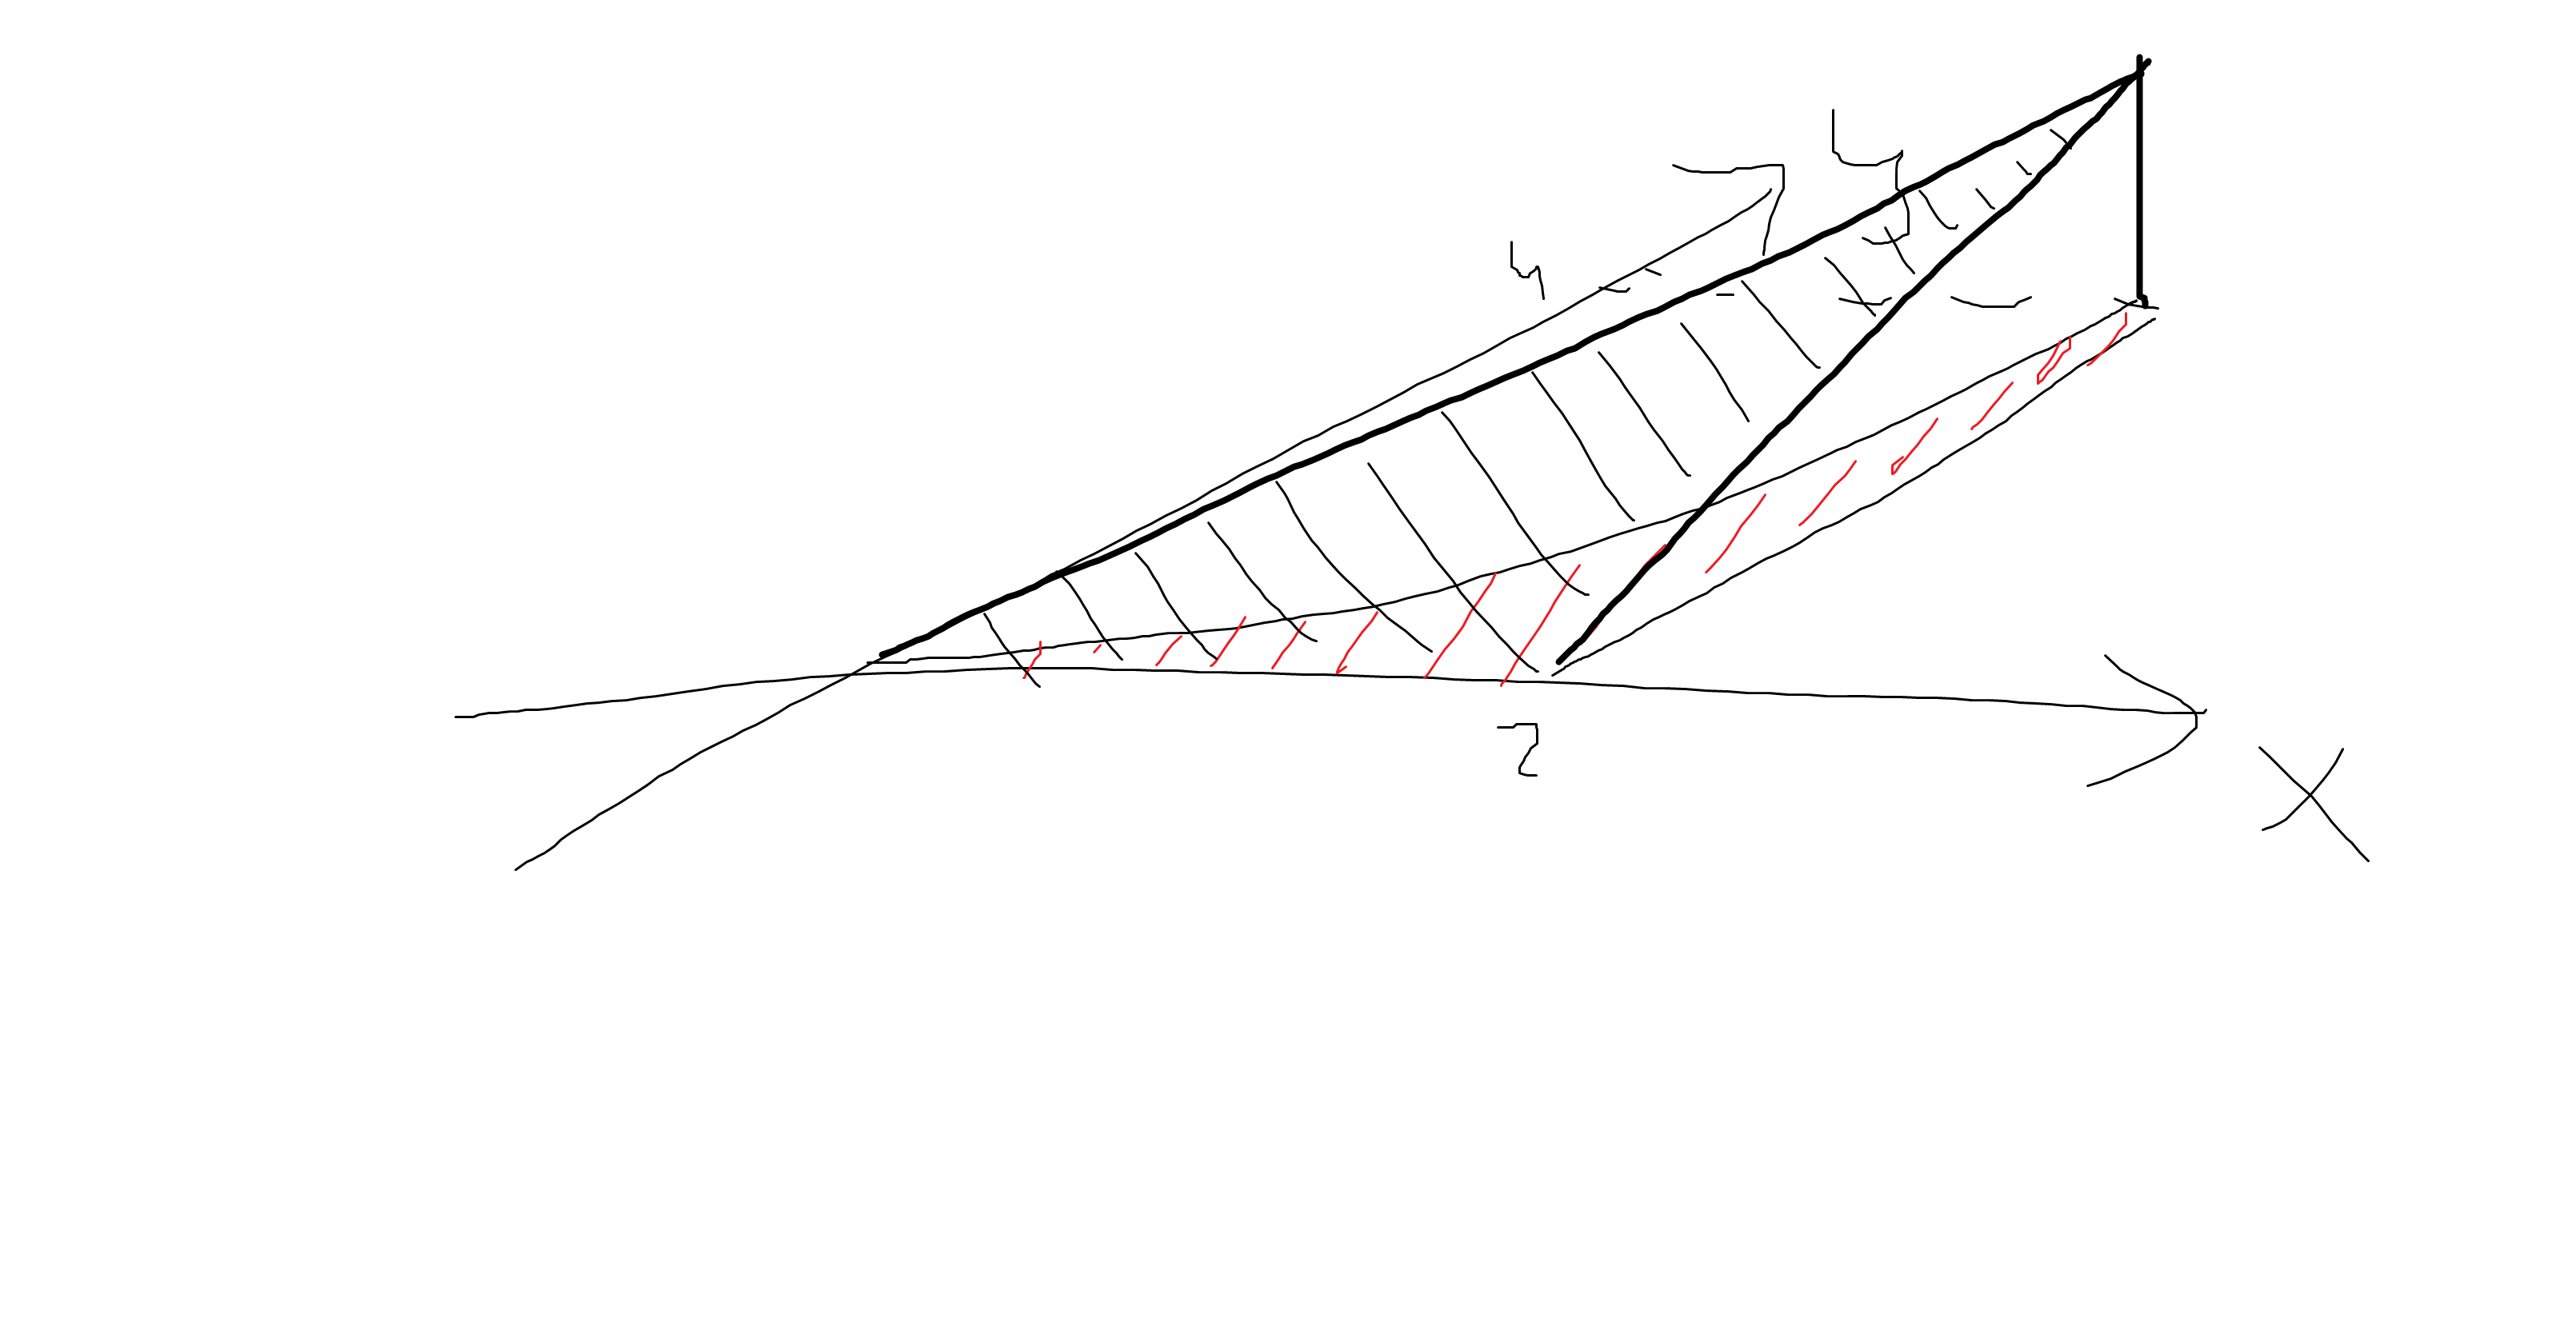
\includegraphics[height=4cm]{kepek/47.png}
			\caption{$A$ halmaz, így nézkez ki, egyenlőre csak egy fiktív ábra}
		\end{figure}
		Erre a problémakörre egy tételünk is van: $f\in C(A)$ és $A\subset\R^2$ korlátos és zárt halmaz ($\Leftrightarrow A$ kompakt): $\exists\min\mathcal{R}_f, \max\mathcal{R}_f$.
		
		Bontsuk szép az A halmazt belső pontokra és határpontokra. Belső pontokban tudunk deriválni, itt ha $f'=0$, akkor ott lehet szélső érték. A határpontoknál vissza kell vezetnünk egyváltozós esetre, és az 1 dimenziós technikákat vesszük elő.
		
		\medskip
		Vizsgáljuk a belső pontokat. Ha $(x,y)\in\Int A$:
		\begin{align*}
			\partial_1f(x,y)&=2y=0\\
			\partial_2f(x,y)&=2x-3=0\\
		\end{align*}
		Ebből a $\left(\frac{3}{2},0\right)$-t kapjuk, azonabn ez nem belső pont: $\left(\frac{3}{2},0\right)\notin\Int A$. Ebből már azt is tudhatjuk, hogy belső pontokban ($\Int A$) nem lehet szélső érték.
		\medskip
		
		Most vizsgáljuk a határpontokat, melyek azon pontok, melyeknek létezik olyan környezete, melyben belső és külső pont is található.
		\begin{figure}[H]
			\centering
			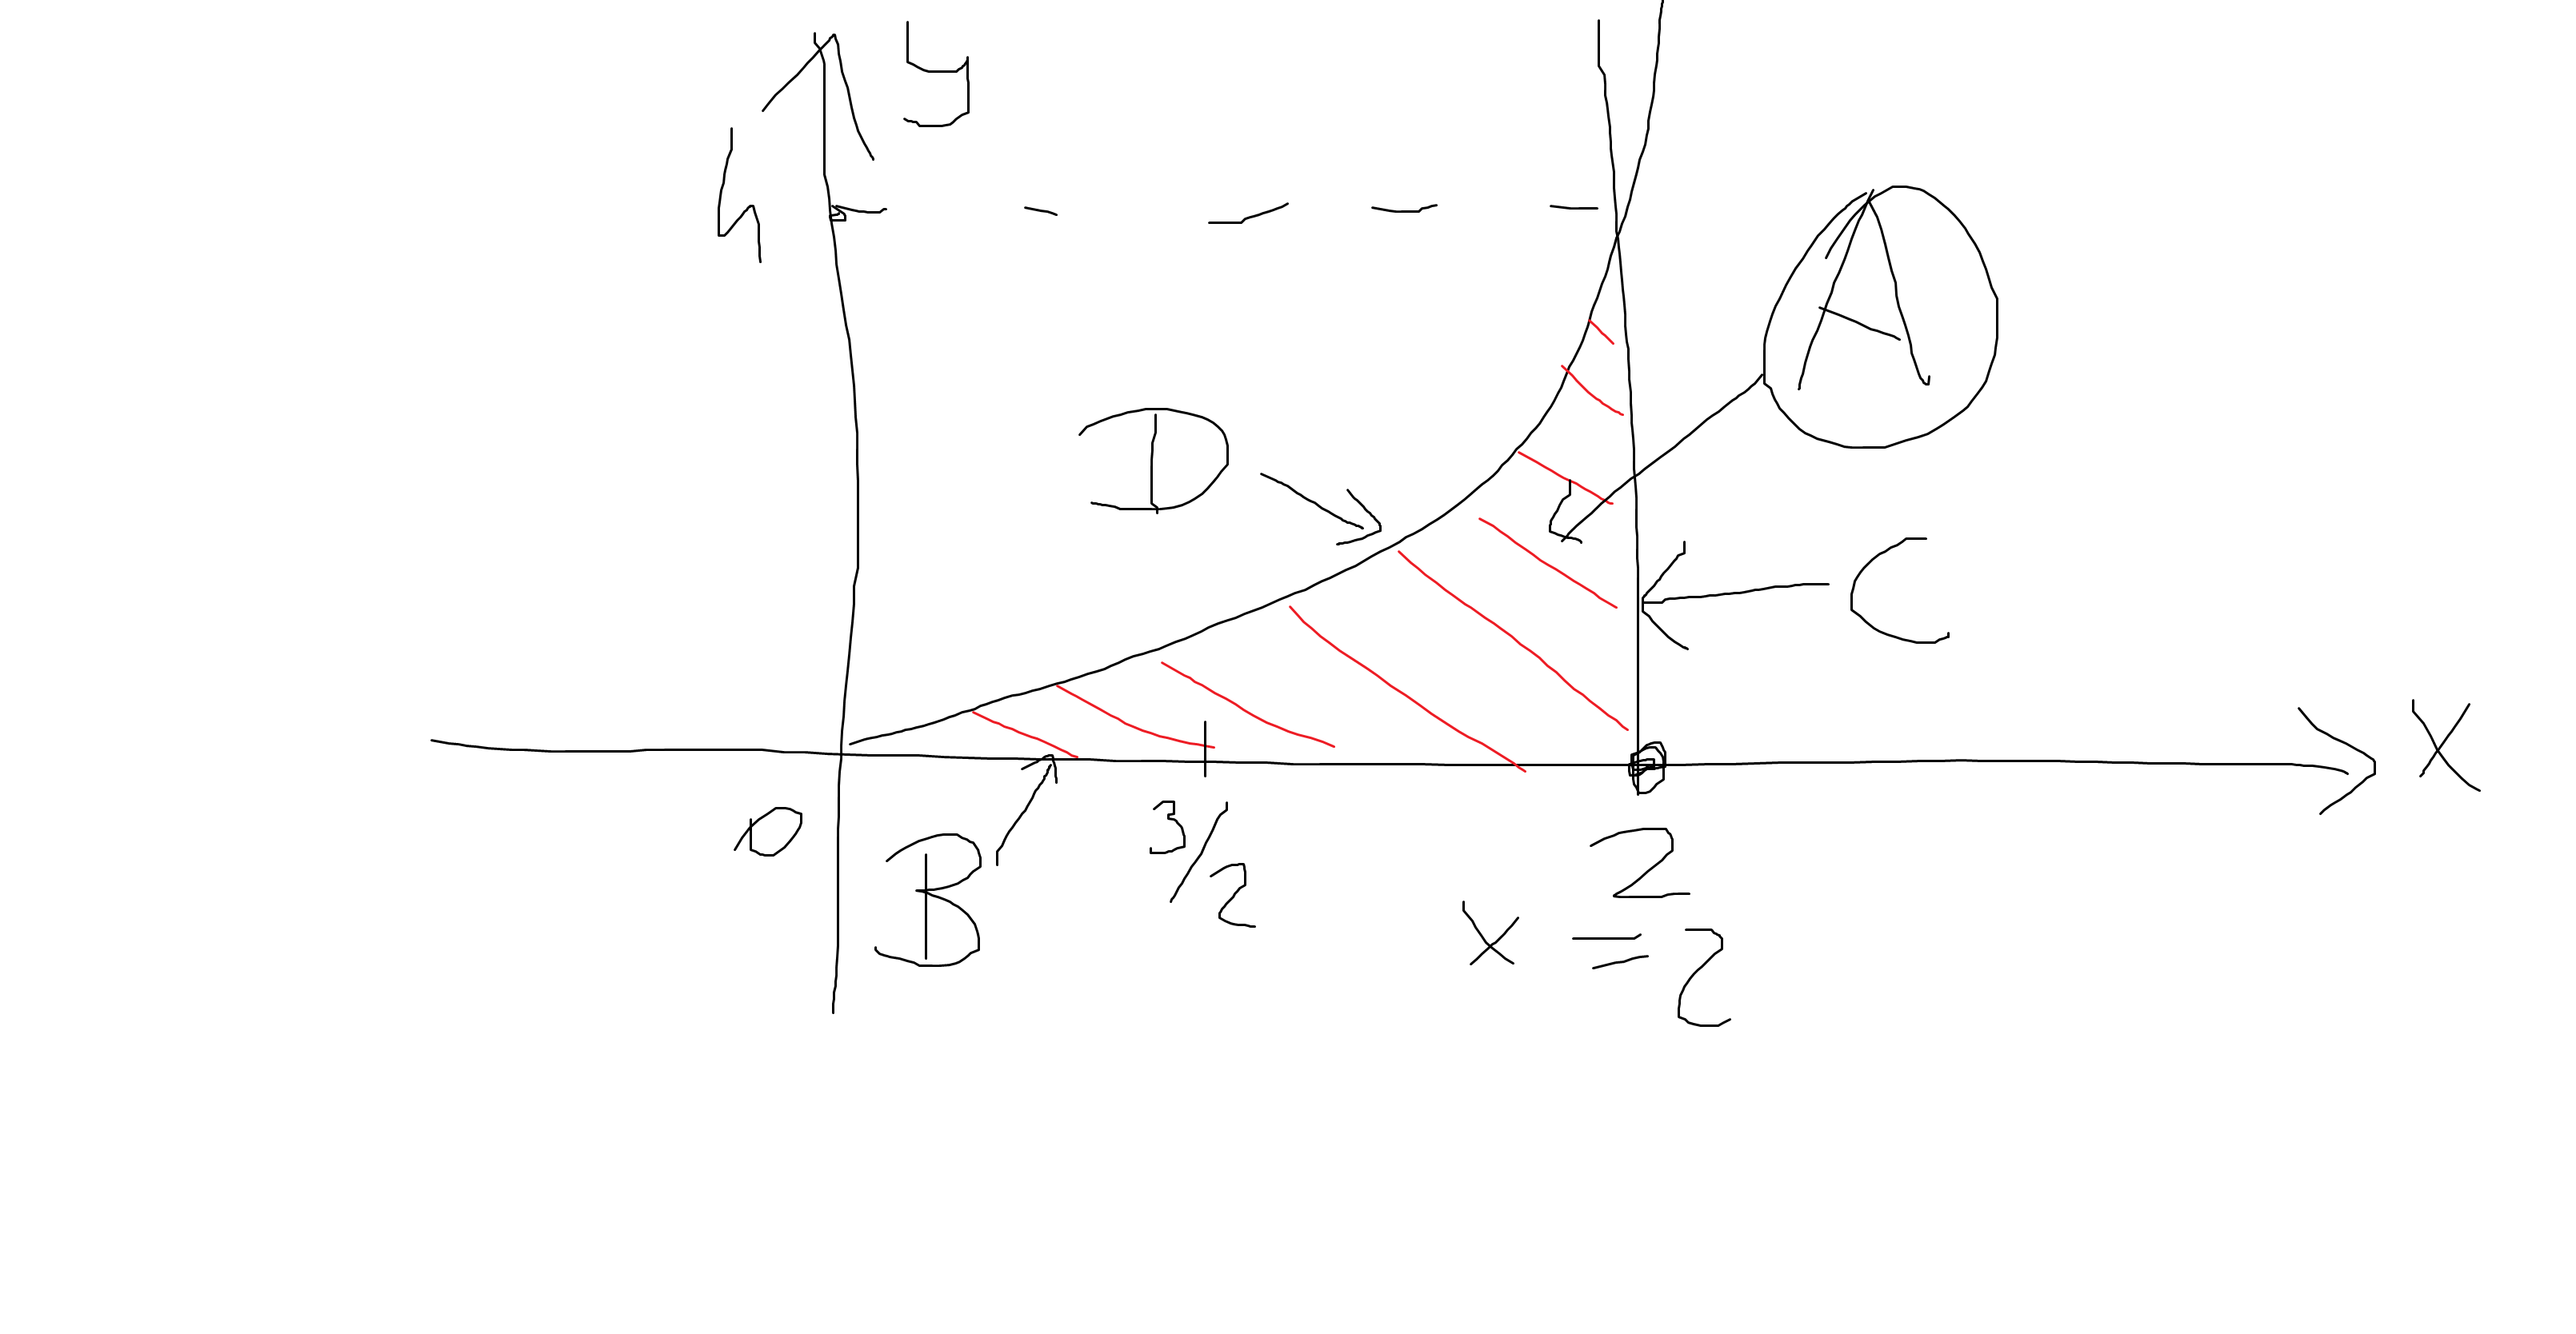
\includegraphics[height=4cm]{kepek/48.png}
			\caption{}
		\end{figure}
		
		$B:=\{(x,0)\in\R^2\ |\ 0\leq x\leq 2 \}$, vizsgáljuk az $f\big|_B$ függvényt!
		\[ g(x):=f(x,0)=0\quad x\in[0,2]\quad \Rightarrow\quad (x,0)\quad (x\in[0,2]) \]
		$C:=\{ (2,y)\in\R^2\ | \ 0\leq y\leq 4 \}$
		\[ h(y):=f(2,y)\quad y\in[0,4] \]
		Ha 
		\[ y\in(0,4)\quad \Rightarrow\quad h'(y)=1\not=0 \]
		$h$ függvény határai: 
		\begin{align*}
			y=0\quad \Rightarrow&\quad (2,0) \quad \text{már volt.}\\
			y=4\quad \Rightarrow&\quad (2,4)
		\end{align*}
		$D:=\{(x,x^2)\in\R^2\ | \ 0\leq x\leq 2\}$
		\[ \Rightarrow\quad l(x):=f(x,x^2)=x^2(2x-3)=2x^3-3x^2\quad x\in[0,2] \]
		Ha $x\in(0,2)\quad \Rightarrow\quad l'(x)=6x^2-6x=6x(x-1)$, ebből pedig $x_1=0\notin(0,2), \quad x_2=1\in(0,2)$ követekezik. Ebből megállapítható, hogy $(1,1)$ lehet szélső érték.
		
		A végpontok, bár mindegyik már megvolt:
		\begin{align*}
			x=0\quad \Rightarrow\quad (0,0)\\
			x=2\quad \Rightarrow\quad (2,4)
		\end{align*}
		
		Harmadik lépésben vessük össze az eddigi eredményeinket.
		\begin{align*}
			f(x,0)=&0\\
			f(2,4)=&4\cdot(2\cdot2-3)=4\quad \text{abszolút maximum}\\
			f(1,1)=&1\cdot(-1)=-1\quad \text{abszolút minimum}\
		\end{align*}
	\end{task}
	\begin{task}
		\[ f(x,y)=x^3-3x^2-y^2 \]
		Legyen
		\[ (x,y)\in A:=\{ (x,y)\in\R^2\ | \ -1\leq x\quad \text{és}\quad x-1\leq y\leq 4 \} \]
		Az ábráról könnyen leolvasható, hogy $x\leq 5$.
		\begin{figure}[H]
			\centering
			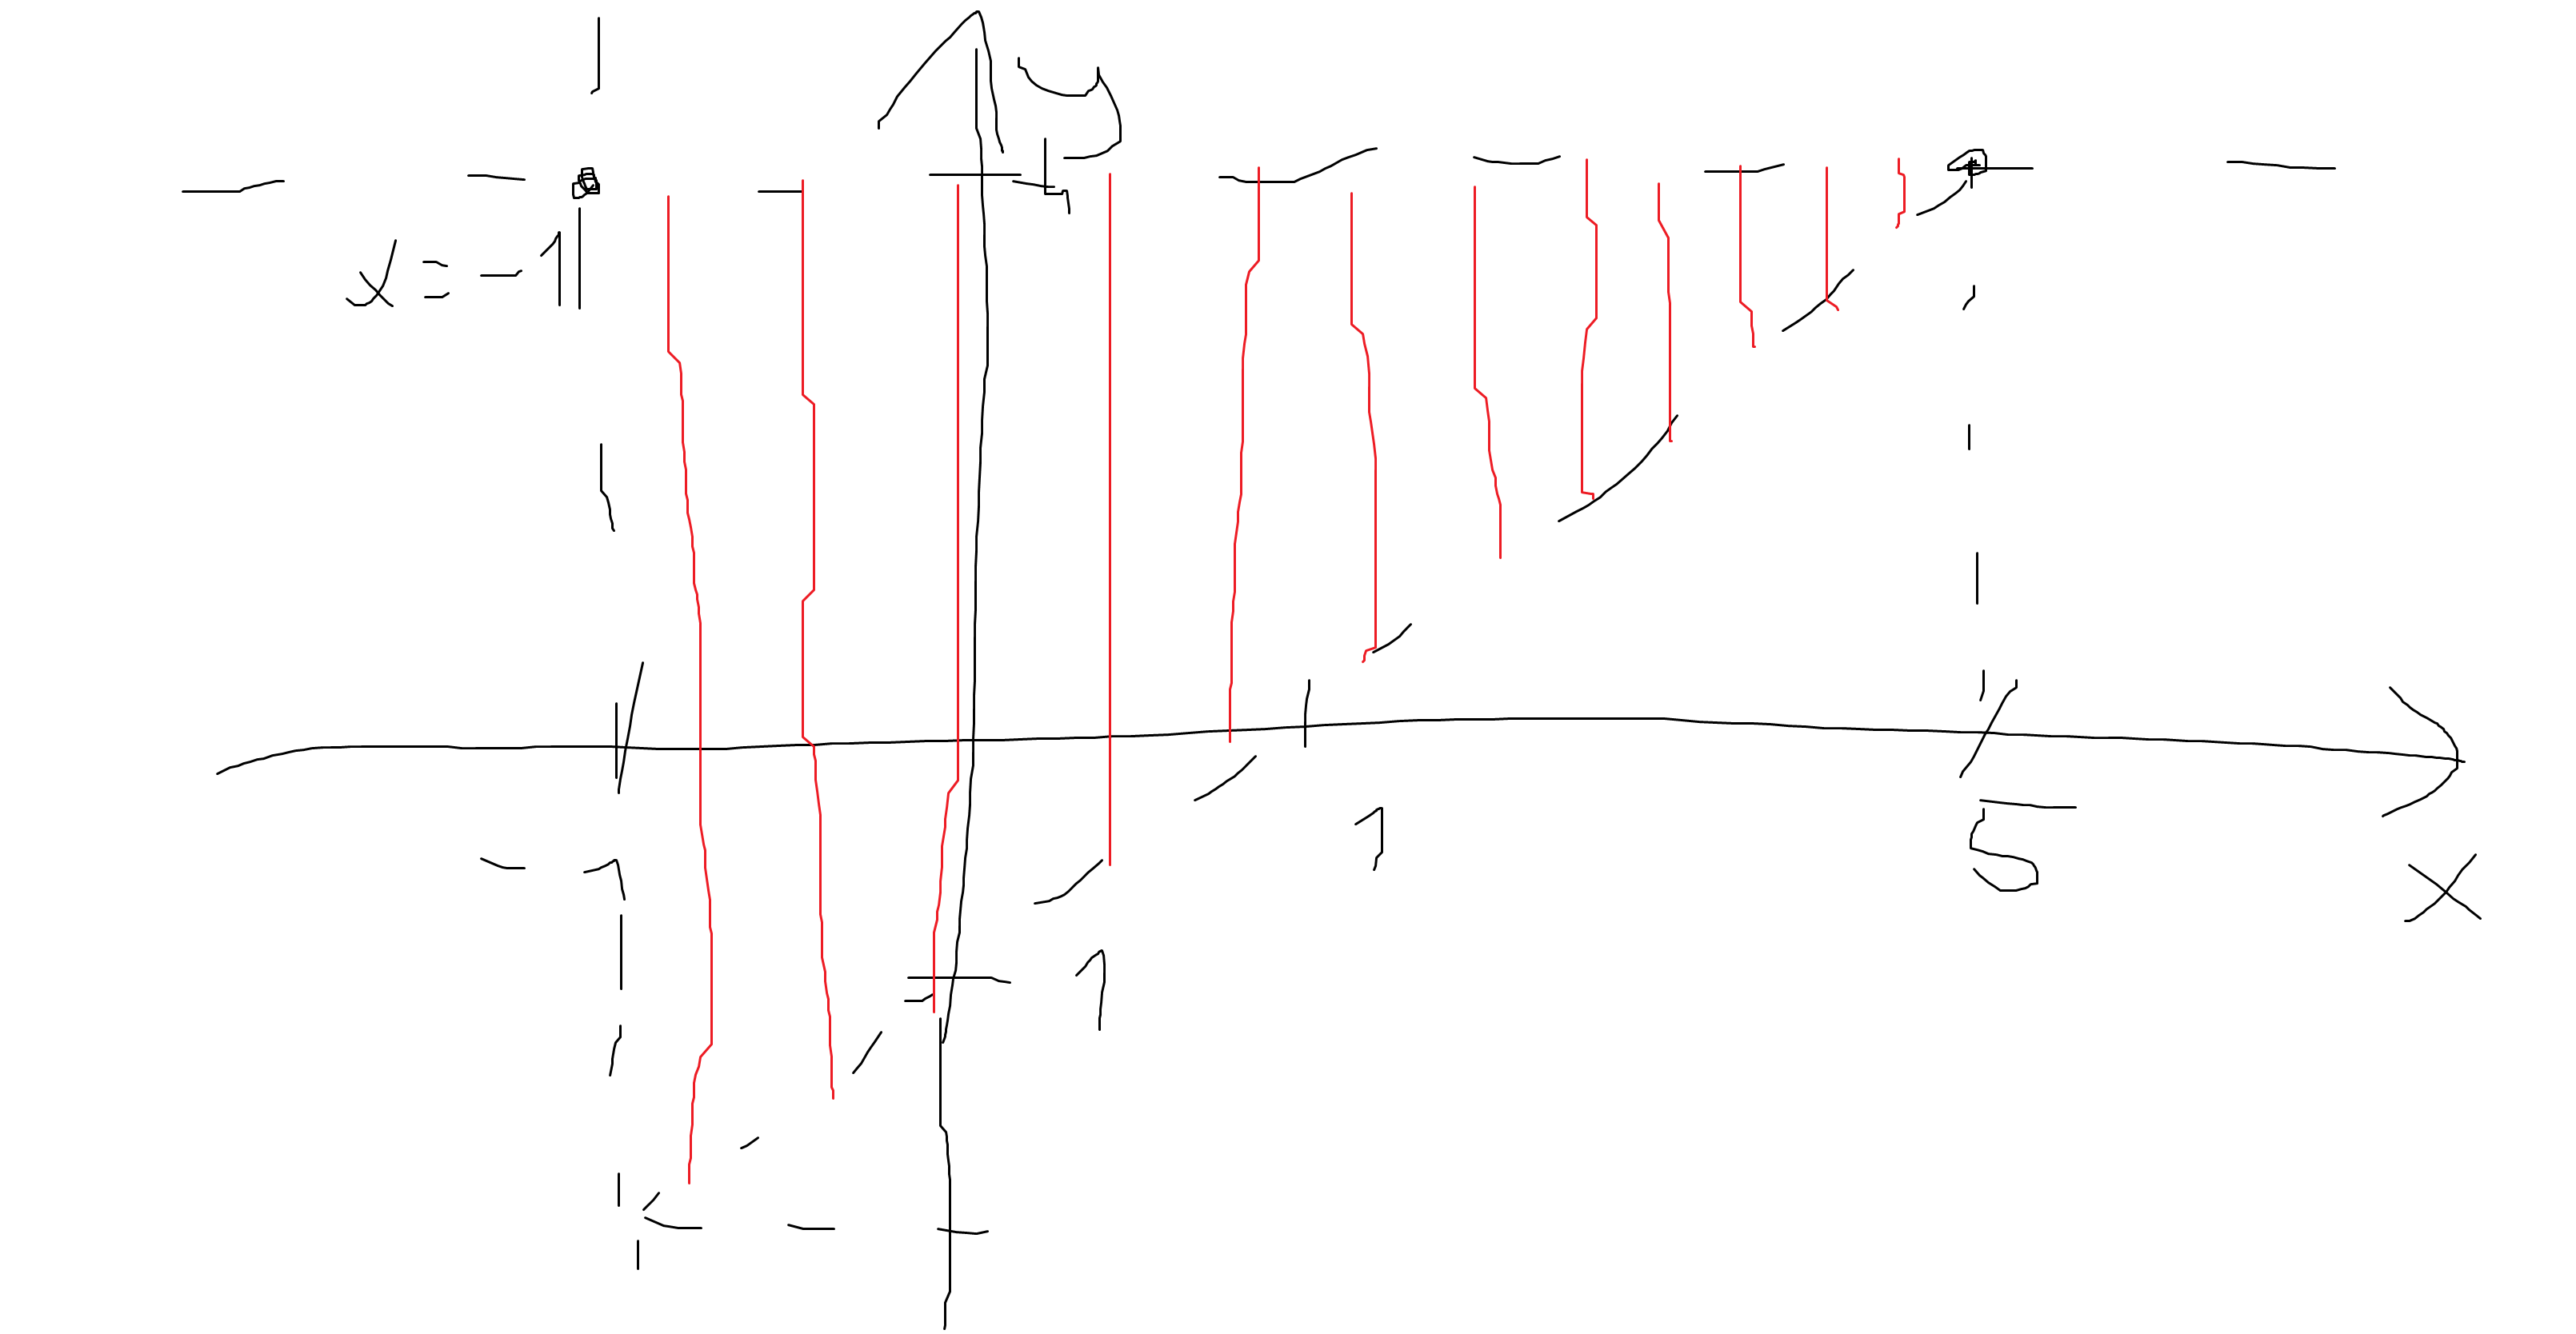
\includegraphics[height=4cm]{kepek/49.png}
			\caption{Az $A$ halmaz}
		\end{figure}
		
		$f\in C(A)$ és $A$ kompakt (korlátos és zárt)\quad $\Rightarrow\quad \exists\min\mathcal{R}_f, \max\mathcal{R}_f$.
		
		Ha $(x,y)\in\Int A\quad \Rightarrow$
		\begin{align*}
			\partial_1f(x,y)&=3x^2-6x=0\\
			\partial_2f(x,y)&=-2y=0
		\end{align*}
		Ebből $x_1=y_1=0$, valamint $x_2=2,\quad y_2=0$ következik. 
		\[ (0,0)\in\Int A,\quad (2,0)\notin\Int A \]
		Így (2,0) nem lehet abszolút szélső érték, (0,0)-t pedig később kell vizsgálnunk.
		
		Most dolgozzunk  határokkal:
		\begin{figure}[H]
			\centering
			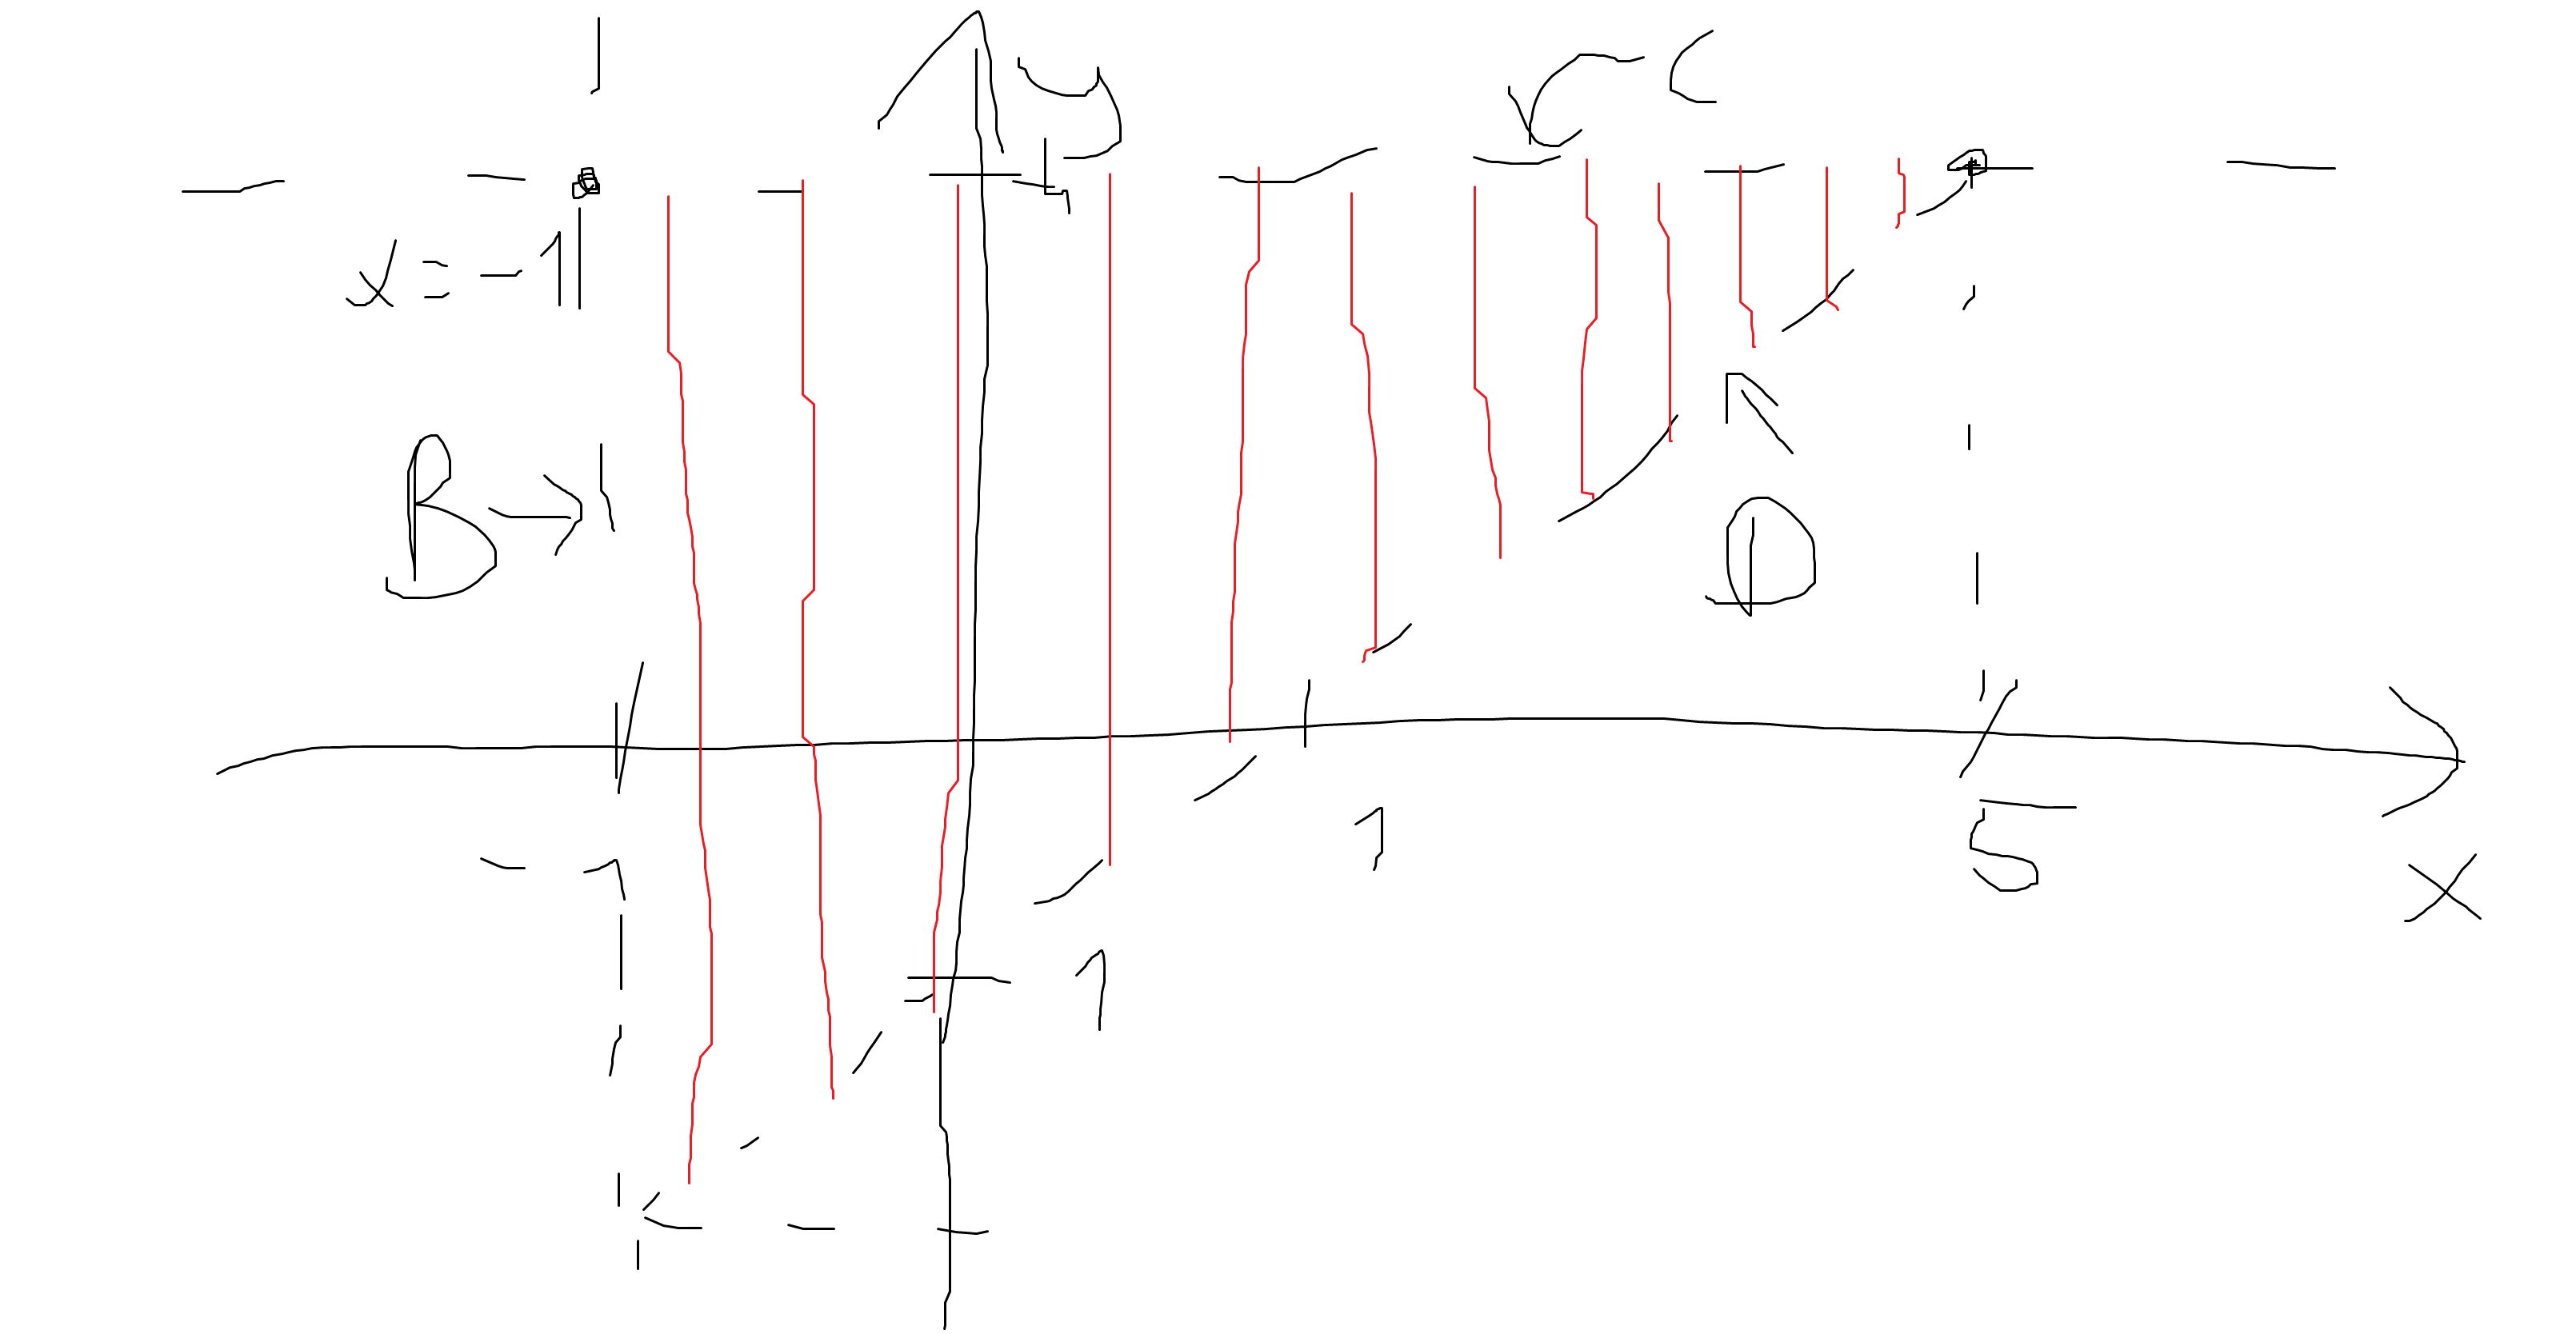
\includegraphics[height=4cm]{kepek/50.png}
			\caption{}
		\end{figure}
		
		
		$B:=\{ (-1,y)\in\R\ | \ -2\leq y\leq 4 \}$
		\[ g(y):=f(-1,y)=-4-y^2\quad y\in[-2,4] \]
		Ha $y\in(-2,4)\quad \Rightarrow\quad g'(y)=-2y=0\quad \Leftrightarrow\quad y=0\in(-2,4)\quad \Rightarrow\quad (-1,0)$.
		
		Végpontok:
		\begin{align*}
			y=-2\quad \Rightarrow&\quad (-1,-2)\\
			y=4\quad \Rightarrow&\quad (-1,4)
		\end{align*}
		Mind a kettő pontot meg kel majd vizsgálunk.
		
		$C:=\{ (x,4)\in\R^2\ | \ -1\leq x\leq 5 \}$
		\[ l(x):=f(x,4)=x^3-3x^2-16\quad x\in[-1,5] \]
		Ha $x\in(-1,5)\quad \Rightarrow\quad l'(x)=3x^2-6x=3x(x-2)=0$, melyből $x_1=0,\quad x_2=2$,\quad $x_1,x_2\in(-1,5)$, azaz (0,4)-et és (2,4)-et is meg kell majd vizsgálni.
		
		Sarokpontok:
		\begin{align*}
			x=-1\quad \Rightarrow&\quad (-1,4)\quad \text{már volt}\\
			x = 5\quad \Rightarrow&\quad (5,4)
		\end{align*}
		$D:=\{ (x,x-1)\in\R^2\ | \ -1\leq x\leq 5 \}$
		\[ h(x):=f(x,x-1)=x^3-3x^2-(x-1)^2\quad x\in[-1,5] \]
		Ha $x\in(-1,5)\quad \Rightarrow h'(x)=3x^2-6x-2(x-1)\cdot1=3x^2-8x+2=0\quad \Leftrightarrow\quad x_1=\frac{4+\sqrt{10}}{3}\in(-1,5), x_2=\frac{4-\sqrt{10}}{3}\in(-1,5)$
		
		sarokpontok:
		\begin{align*}
			\left(\frac{4+\sqrt{10}}{3},\frac{1+\sqrt{10}}{3}\right)\\
			\left(\frac{4-\sqrt{10}}{3},\frac{1-\sqrt{10}}{3}\right)
		\end{align*}
		
		Vessük össze:
		\begin{figure}[H]
			\centering
			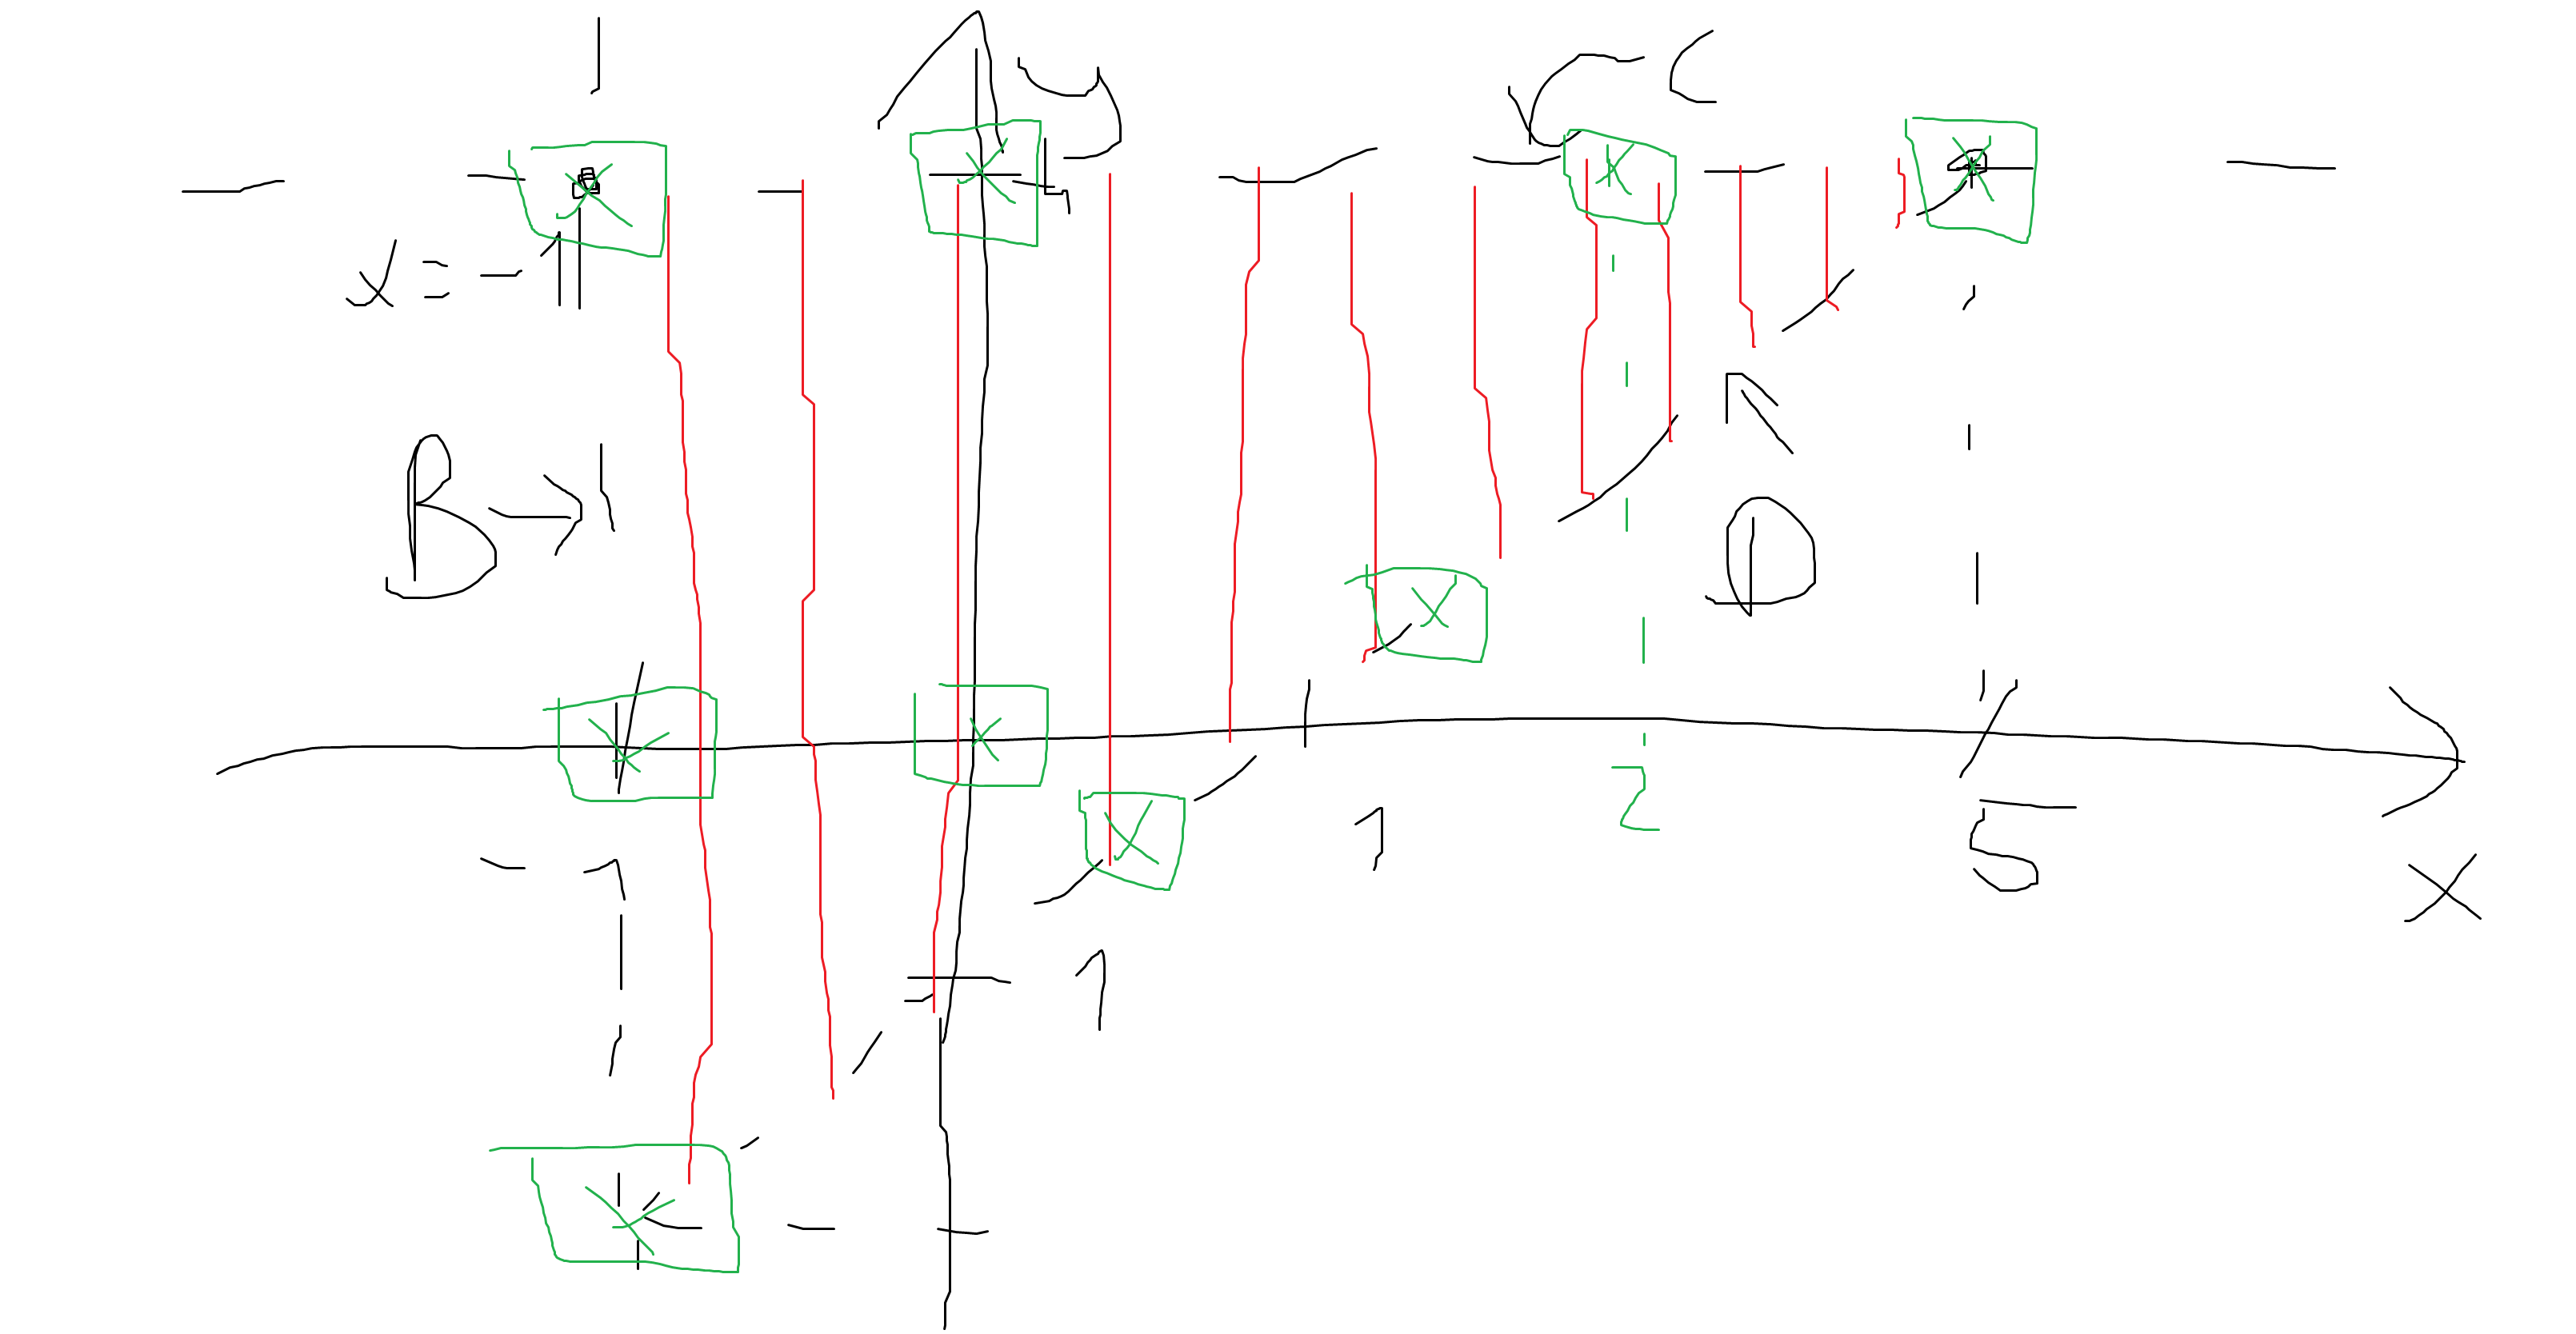
\includegraphics[height=4cm]{kepek/51.png}
			\caption{}
		\end{figure}
		\begin{align*}
			f(0,0)&=0\\
			f(-1,-2)&=-8\\
			f(-1,0)&=-4\\
			f(-1,4)&=-20\quad \text{abszolút minimum}\\
			f(0,4)&=-16\\
			f(2,4)&=-20\quad \text{abszolút minimum}\\
			f(5,4)&=34\quad \text{abszolút maximum}\\
			f\left(\frac{4+\sqrt{10}}{3},\frac{1+\sqrt{10}}{3}\right)&=\text{HF}, \in(-20,34)\\
			f\left(\frac{4-\sqrt{10}}{3},\frac{1-\sqrt{10}}{3}\right)&=\text{HF} \in(-20, 34)
		\end{align*}
	\end{task}
	\begin{note}
		Az $A$ halmaz ábrázolása 1 pont, a Weierstass tétel felírása 1 pont, a deriváltak felírása (ált.) 2 pont, a határvonalak 1-2 pontot érnek darabonkéntösszevetés 1pont
	\end{note}
\end{document}